% Beamer Presentation and Lecture Note Template
% Version 0.1
% by Paul Vesey

\mode<presentation> {
\usetheme{Antibes}
\setbeamercovered{invisible}
\setbeamertemplate{footline}[frame number]
\setbeamertemplate{navigation symbols}{} 
}

\usepackage{eurosym}
\usepackage{graphicx}
\usepackage{wasysym}
\usepackage{hyperref}
\usepackage{amsmath}
\usepackage{amssymb}
\usepackage{mathtools}
\usepackage{tikz}
\usepackage{pgf}
\usepackage{pgfplots}
\usepackage{pxfonts}
\usepackage{textcomp}
\usepackage{verbatim}
\usepackage{color}
\usepackage{xcolor}
\usepackage{fix-cm}


\author{Paul Vesey}
\institute[TUS]
{
Technological University of the Shannon \\
\medskip
{\emph{paul.vesey@tus.ie}}
}
\date{Autumn 2022}


%
\title[Project Management \& BIM]{Project Cost Management}


\begin{document}
%

\tableofcontents
\newpage



\begin{frame}
\titlepage
\end{frame}
\begin{center}\line(1,0){250}\end{center}
%
%


\section{Project Cost Management}

\subsection{Introduction}


\begin{frame}
\frametitle{Project Cost Management}
Consists of 3 Processes\\
\begin{enumerate}
	\item Estimate Cost
	\item Determine Budget
	\item Control Costs
\end{enumerate}
Project Cost Management is primarily concerned with the cost of resources needed to complete schedule activities\\
\textbf\textit{Project Cost Management is not the same as Life-Cycle Costing}\\
\end{frame}
\begin{center}\line(1,0){250}\end{center}


\begin{frame}
\frametitle{Project Cost Management}
\textbf{Estimate Costs}
\begin{itemize}
	\item Developing an approximation of the costs of the resources needed to complete project activities
\end{itemize}
\textbf{Determine Budget}
\begin{itemize}
	\item Aggregating the estimated costs on individual activities or work packages to establish a cost baseline
\end{itemize}
\textbf{Control Costs}
\begin{itemize}
	\item Influencing the factors that create cost variances and controlling changes to the project budget
\end{itemize}
\end{frame}
\begin{center}\line(1,0){250}\end{center}





\begin{frame}
\frametitle{Project Cost Management}
Different stakeholders will measure project costs in different ways; this can have a major effect on finance reporting
\begin{itemize}
	\item Typically these variances will be on how costs are booked to the project.

	\item e.g. Large AHU's (over \euro20k) may be booked to the project when the order is placed, and a portion of the bill item may be invoiced to the client when the equipment is delivered to site.
\end{itemize}
\end{frame}
\begin{center}\line(1,0){250}\end{center}







\begin{frame}
\frametitle{Project Cost Management}
On small projects Estimating Costs and Determining Budget are sometimes so closely linked that determining where one finished and the other starts is virtually impossible\\
This would rarely (if ever) apply to construction contracts.
\begin{itemize}
	\item Estimating is carried out at tender stage; budgeting at construction stage
	\item Typically, construction firms struggle with cash-flow due to the time between incurring costs associates with work, and actually getting paid for it.
	\item Most construction contracts have a retention clause (circa 5\%) which needs to be considered in cash flow projections and Earned Value Analysis. 
\end{itemize}
\end{frame}
\begin{center}\line(1,0){250}\end{center}






\begin{frame}
\frametitle{Project Cost Management}
\textbf{Early stages of a project have the greatest influence in the overall costs associated with a project}
\begin{itemize}
	\item This is one of the main reasons why correctly 'scoping' a project is so important.
\end{itemize}
Construction Projects can have difficulty with this aspect, especially when consideration is given to the concept of 'progressive elaboration'; something that is inherent in construction projects\\
Scope Creep is another issue that needs to be watched\ldots
\end{frame}
\begin{center}\line(1,0){250}\end{center}






\begin{frame}
\frametitle{Cost Management Plan}
\textbf{Establishes the Precision Level to be used for cost estimates}
\begin{itemize}
	\item Nearest \euro100, \euro1000, etc.
\end{itemize}
\textbf{Defines Units of Measure}
\begin{itemize}
	\item staff-hours, staff-weeks, lump sum etc.
\end{itemize}
\textbf{Control Accounts}
\begin{itemize}
	\item As per WBS
\end{itemize}
\textbf{Control Thresholds}
\begin{itemize}
	\item Limits to acceptable variations against budgeted figures
\end{itemize}
\end{frame}
\begin{center}\line(1,0){250}\end{center}






\begin{frame}
\frametitle{Cost Management Plan}
\textbf{Performance Measurement Rules}
\begin{itemize}
	\item Earned Value Management formulas
	\item WBS level to which Earned Value analysis will be applied
	\item Etc.
\end{itemize}
\textbf{Reporting Formats}\\
\textbf{Process Descriptions}
\end{frame}
\begin{center}\line(1,0){250}\end{center}






\begin{frame}
\frametitle{Project Cost Management \hfill Points to Consider}
\textbf{Cost Management is not Cost Monitoring}
\begin{itemize}
	\item Just because you know how much cost has been incurred (or booked) to a project, it does not necessarily mean you are in control of the situation
\end{itemize}
Poor cash flow can kill a company.\\
If a project is due to run for a considerable length of time, longer than 12 months, pay particular attention to the CPA clause.
	\begin{itemize}
		\item Be wary of links to the Consumer Price Index; it may not represent your actual increases in cost
		\item Better to look for:
		\begin{itemize}
			\item Table 1 - Average Earnings and Hours Worked by Skilled and Unskilled Operatives for Earnings and Hours worked in Construction
			\item Table 3 - Wholesale Price Indices (excluding VAT) for Building and Construction Materials from the Wholesale Price Index
		\end{itemize}
	\end{itemize}
\end{frame}
\begin{center}\line(1,0){250}\end{center}







\begin{frame}
\frametitle{Project Cost Management}
Example CPA table
\begin{figure}
	\centering
		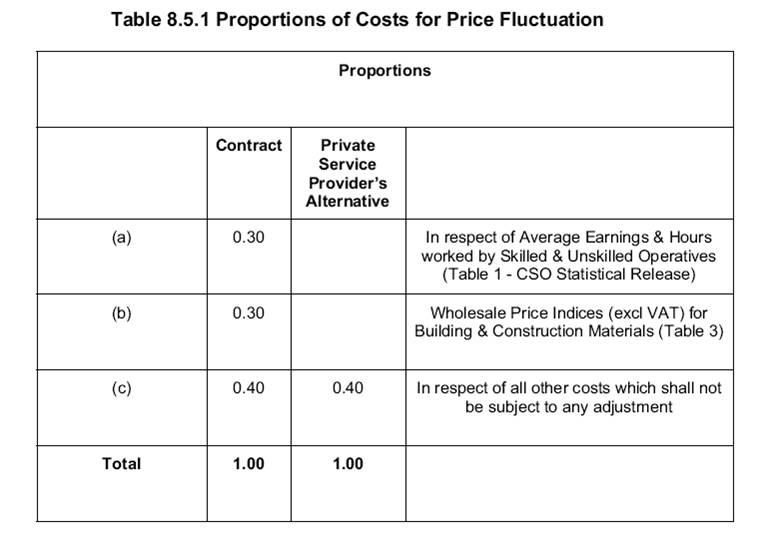
\includegraphics[width = 8cm]{images/CPA.jpg}
	\caption{CPA Table}
	\label{fig:CPA}
\end{figure}
\end{frame}
\begin{center}\line(1,0){250}\end{center}






\begin{frame}
\frametitle{Effects of Inflation}
 \begin{figure}
 	\centering
 		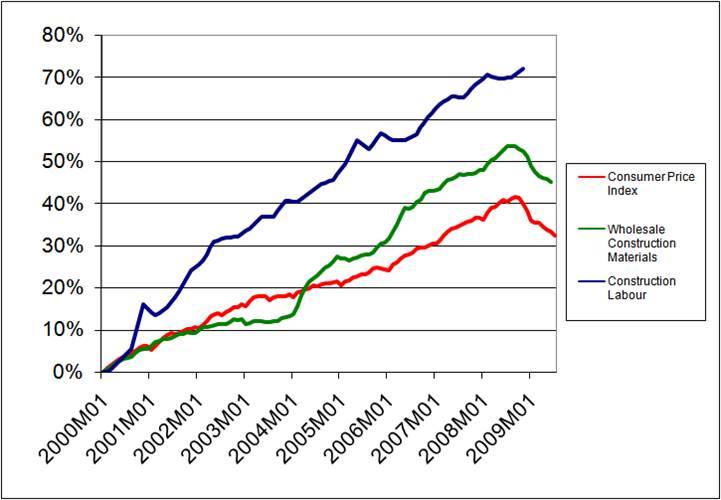
\includegraphics[width = 10cm]{images/deflation.jpg}
 	\label{fig:deflation}
 \end{figure}
\end{frame}
\begin{center}\line(1,0){250}\end{center}






\begin{frame}
\frametitle{Estimate Costs}
\begin{figure}
	\centering
		\includegraphics[width = 8cm]{images/fig7-4.jpg}
	\label{fig:7-4}
\end{figure}Part of the Planning Process Group
\end{frame}
\begin{center}\line(1,0){250}\end{center}






\begin{frame}
\frametitle{Estimate Costs}
\textbf{Cost Estimating is not the same as Pricing}\\
\begin{itemize}
	\item Pricing is concerned with what you should pay
	\item Cost estimating is concerned with what an activity will actually cost the performing organisation
\end{itemize}
\textbf{Inputs}\\
\begin{itemize}
	\item As per book
	\item Enterprise Environmental Factors (Marketplace Conditions)
	\item What is available, from whom, and under what terms and conditions
	\begin{itemize}
		\item Published Commercial Information. May be an electronic database (CSO) or printed (SPON)
	\end{itemize}
	\item Information on skills and labour costs
\end{itemize}
\end{frame}
\begin{center}\line(1,0){250}\end{center}









\begin{frame}
\frametitle{Inputs \hfill Organisational Process Assets}
\textbf{Cost Estimating Policies}
\begin{itemize}
	\item Predefined approaches and rules for cost estimating
	\item Typically generated by finance department or PMO
\end{itemize}
\textbf{Cost Estimating Templates}
\begin{itemize}
	\item Standardised forms and methods
	\item Can be restrictive; but lessen the likelihood of omissions
	\item For best effect, they need to be flexible
\end{itemize}
\textbf{Historical Information}
\begin{itemize}
	\item The performing organisations experiences may influence costing
	\item Files from previous projects of a similar nature can be reviewed for costing techniques and validation of estimated costs
	\item Project Team Knowledge
\end{itemize}
\end{frame}
\begin{center}\line(1,0){250}\end{center}








\begin{frame}
\frametitle{Inputs \hfill\hfill Organisational Process Assets}
\textbf{Lessons Learned}
\begin{itemize}
	\item - Lessons learned from previous projects of a similar nature
	\item Project Scope Statement: Includes information that is likely to impact cost estimates
		\begin{itemize}
			\item Constraints, Assumptions, Requirements, Etc.
			\item Also contains deliverables and acceptance criteria: these must be considered when estimating cost.
		\end{itemize}
\end{itemize}
\textbf{Technical Issues and Concerns}
\begin{itemize}
	\item again, likely to influence cost 
\end{itemize}
\end{frame}
\begin{center}\line(1,0){250}\end{center}







\begin{frame}
\frametitle{Inputs \hfill\hfill Project Schedule}
\begin{itemize}
	\item The types and quantities of resources, and the amount of time they are applied clearly makes up the most significant element of a cost estimate.
	\item 'Estimate Activity Resources' and 'Activity Duration Estimates' provide key information for cost estimation
	\item Most construction projects run for 6-months or more; financing, interest rates, Contract Price Adjustment (CPA) will have a significant effect
	\item Consideration should also be given to time-sensitive cost estimates  
\end{itemize}
\end{frame}
\begin{center}\line(1,0){250}\end{center}






\begin{frame}
\frametitle{Tools and Techniques}
\textbf{Analogous Estimating}
\begin{itemize}
	\item Using actual costs from a similar project to estimate costs for current project
\end{itemize}
\textbf{Determine Resource Cost Rates}
\begin{itemize}
	\item Staff Cost per hour
	\item Material Bulk Cost, $m^{3}$, $m^{2}$, etc.
	\item Quotations
	\item SPON etc
\end{itemize}
\textbf{Bottom-up Estimating}
\begin{itemize}
	\item Involves estimating costs to the lowest levels of the WBS (work packages)
\end{itemize}
\end{frame}
\begin{center}\line(1,0){250}\end{center}






\begin{frame}
\frametitle{Tools and Techniques}
\textbf{Parametric Estimating}
\begin{itemize}
	\item Parametric Estimating involves using the relationship between historical data and other variables to generate an estimate
	\begin{itemize}
		\item i.e. data: average cost of concrete over the last 12 months is \euro72.00 per $m^{3}$
		\item Variable: estimate requires 1000$m^{3}$ of concrete
		\item Cost Estimate for Concrete \euro72,000
		\item Should also include an ``x-factor'' to cover inflation, profit, etc.
	\end{itemize}
\end{itemize}

\end{frame}
\begin{center}\line(1,0){250}\end{center}



\begin{frame}
\frametitle{Tools and Techniques}
 
\textbf{Vendor Bid Analysis}
	\begin{itemize}
		\item Solicitation of quotations for various project elements from a number of sources.
		\item These are then analysed to assist in determining cost
		\item Note: It is not always a good idea to use the lowest figures obtained.  Better to analyse properly and determine an average or consensus figure at tender stage. (Why?)
	\end{itemize}
\end{frame}
\begin{center}\line(1,0){250}\end{center}


\begin{frame}
\frametitle{Tools and Techniques}
\textbf{Reserve Analysis}
\begin{itemize}
	\item AKA Contingency Sums : for use on 'known-unknowns' identified in the scope or during risk management
	\item Can inflate project prices; impacts competitiveness
\end{itemize}
\textbf{Project Management Estimating Software}
\begin{itemize}
	\item Cost Estimating elements of PM software
	\item Can also be spreadsheets, specialist estimating software, Buildsoft, etc. 
\end{itemize}
\end{frame}
\begin{center}\line(1,0){250}\end{center}






\begin{frame}
\frametitle{Project Management Software}
MS Project Example
\begin{figure}
	\centering
		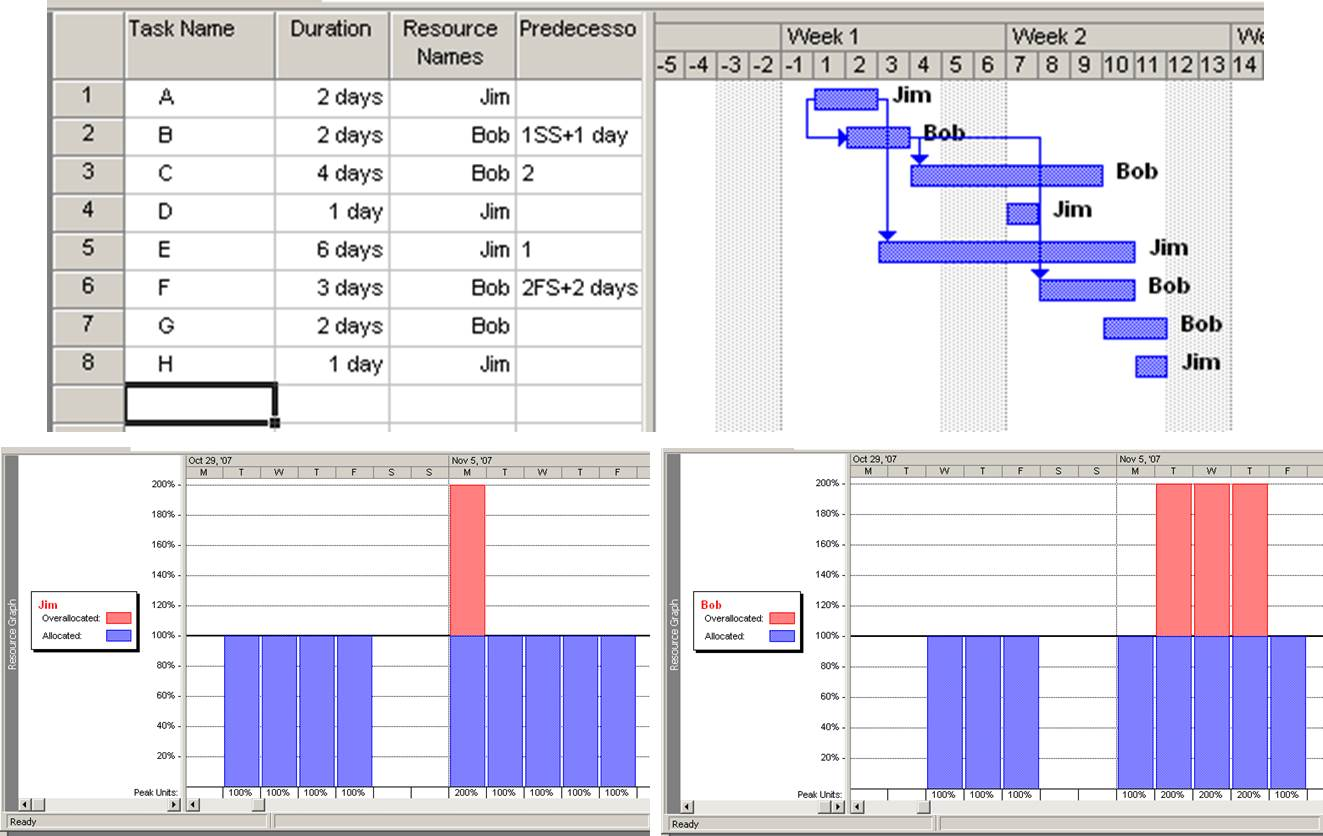
\includegraphics[width = 10cm]{images/msprojres.jpg}
	\label{fig:msprojres}
\end{figure}
\end{frame}
\begin{center}\line(1,0){250}\end{center}











\begin{frame}
\frametitle{Resource Leveling}
Resource Graph (View | Resource Graph)
\begin{figure}
	\centering
		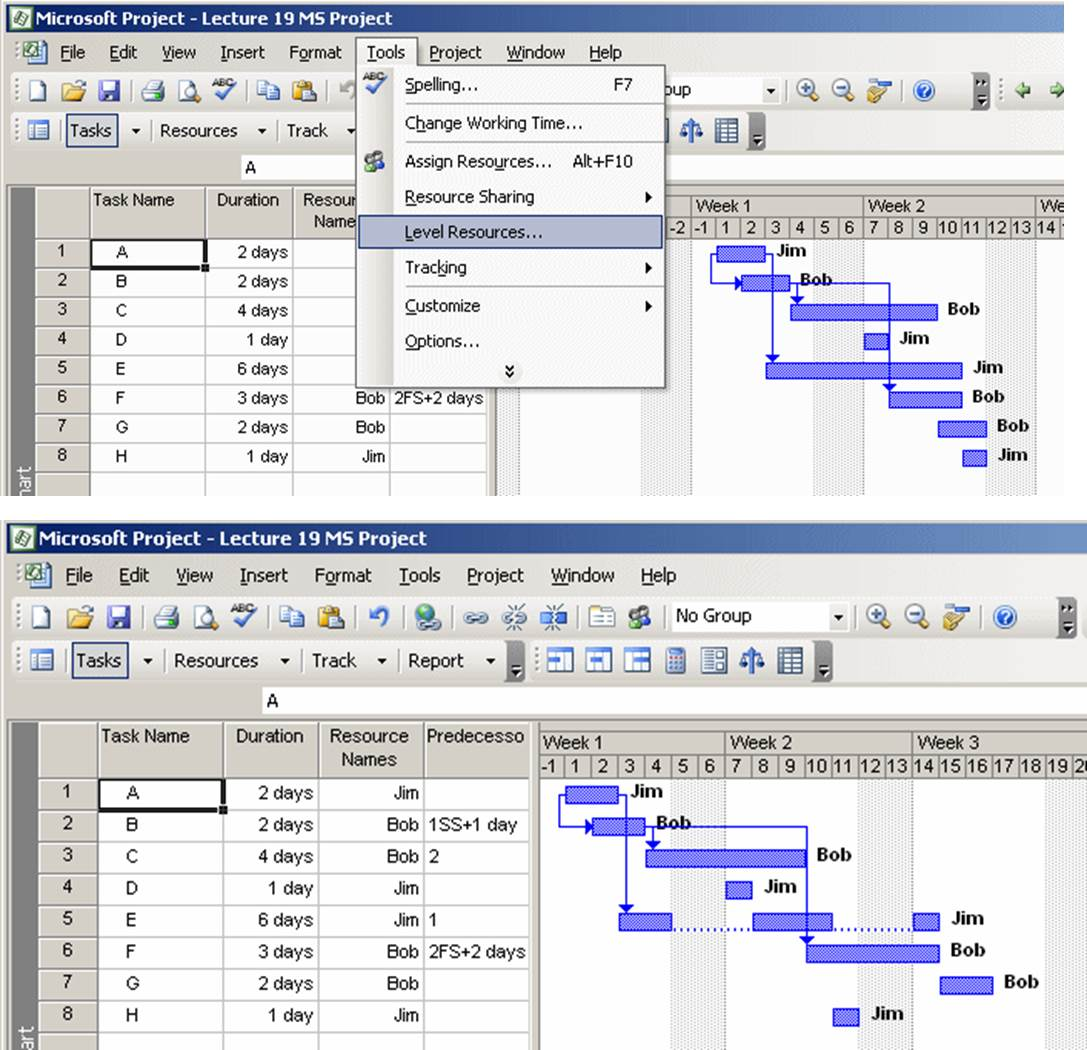
\includegraphics[width = 6cm]{images/reslevel.jpg}
	\label{fig:reslevel}
\end{figure}
\end{frame}
\begin{center}\line(1,0){250}\end{center}






\begin{frame}
\frametitle{Resource Leveled}
\begin{figure}
	\centering
		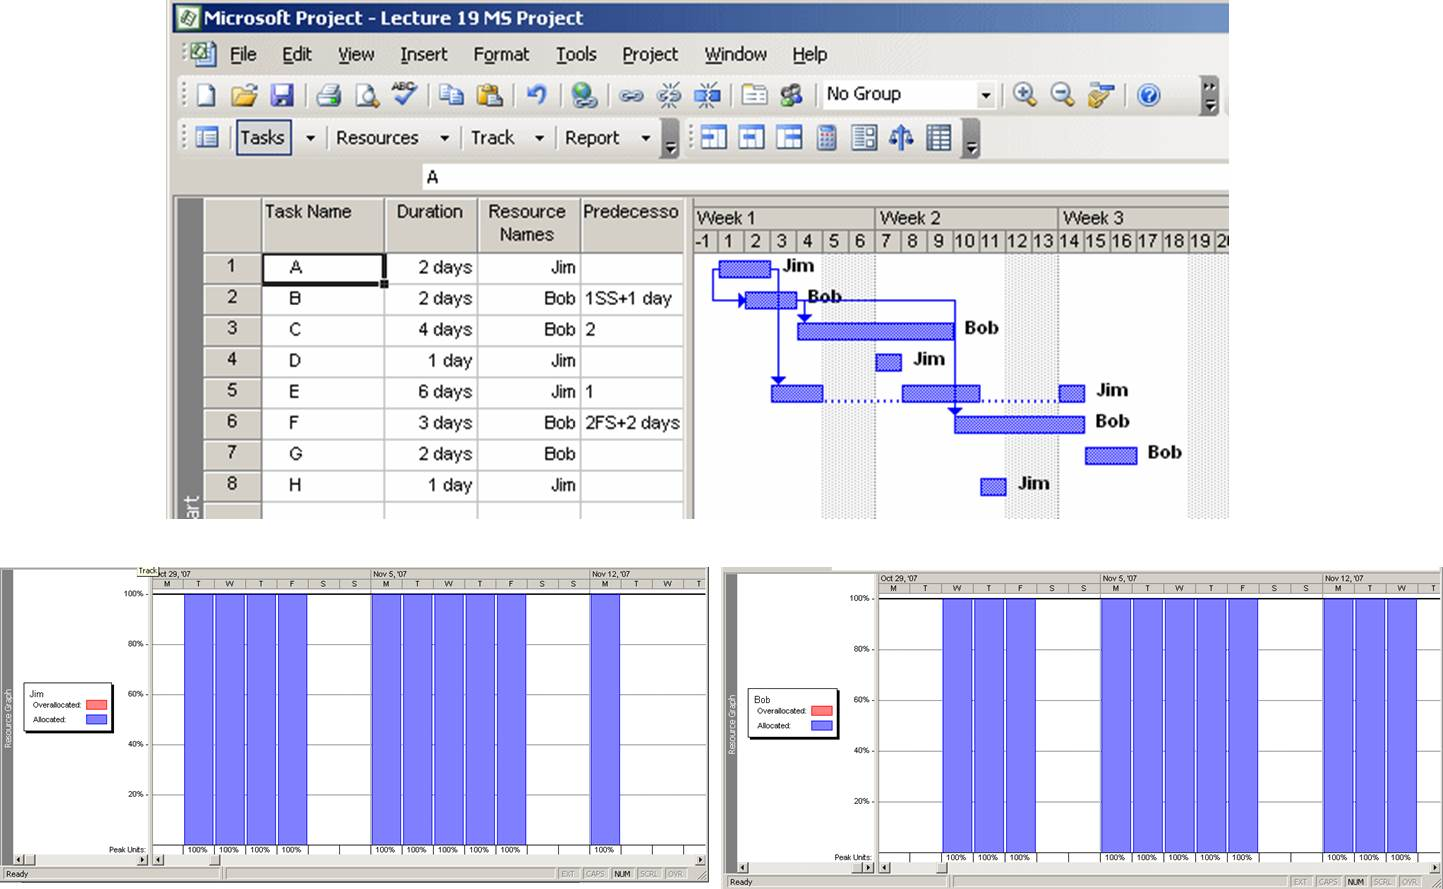
\includegraphics[width = 10cm]{images/resleveled.jpg}
	\label{fig:resleveled}
\end{figure}

\end{frame}
\begin{center}\line(1,0){250}\end{center}






\begin{frame}
\frametitle{MS Project}
View | Resource Sheet\\\begin{figure}
	\centering
		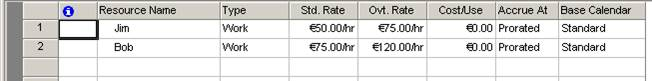
\includegraphics[width = 10cm]{images/ressheet.jpg}
	\label{fig:ressheet}
\end{figure}


View | Table : Cost\\\begin{figure}
	\centering
		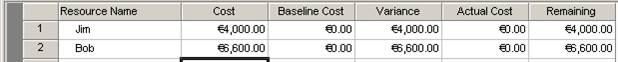
\includegraphics[width = 10cm]{images/costsheet.jpg}
	\label{fig:costsheet}
\end{figure}


View | Gantt Chart then| View | Table : Cost\\\begin{figure}
	\centering
		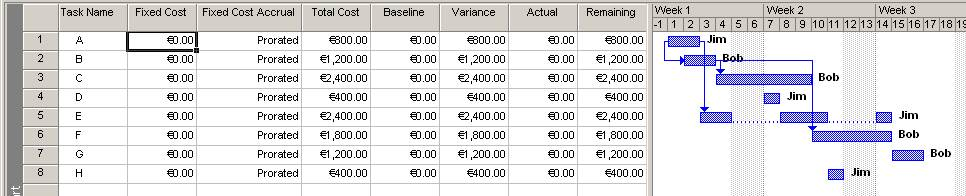
\includegraphics[width = 10cm]{images/ganttcost.jpg}
	\label{fig:ganttcost}
\end{figure}
\end{frame}
\begin{center}\line(1,0){250}\end{center}







\begin{frame}
\frametitle{MS Project}
View | Task Usage\\\begin{figure}
	\centering
		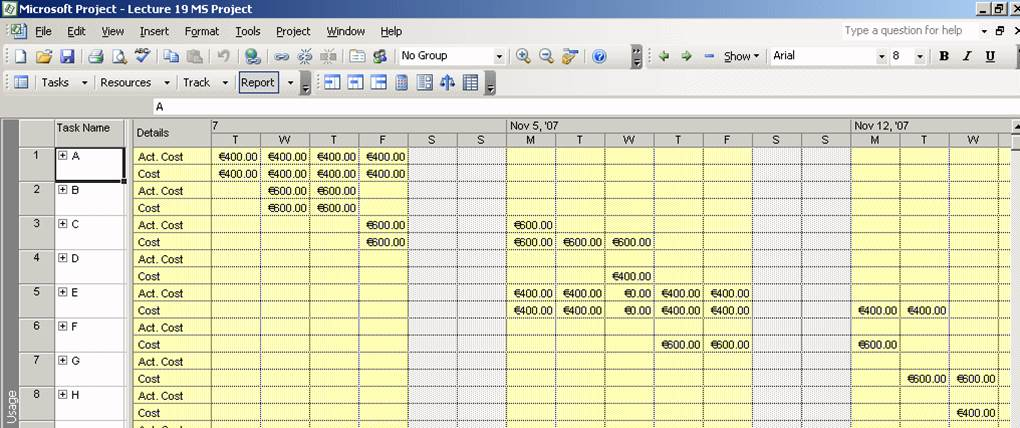
\includegraphics[width = 10cm]{images/costtrack.jpg}
	\label{fig:costtrack}
\end{figure}
\end{frame}
\begin{center}\line(1,0){250}\end{center}






\begin{frame}
\frametitle{}
Imported to Excel
\begin{figure}
	\centering
		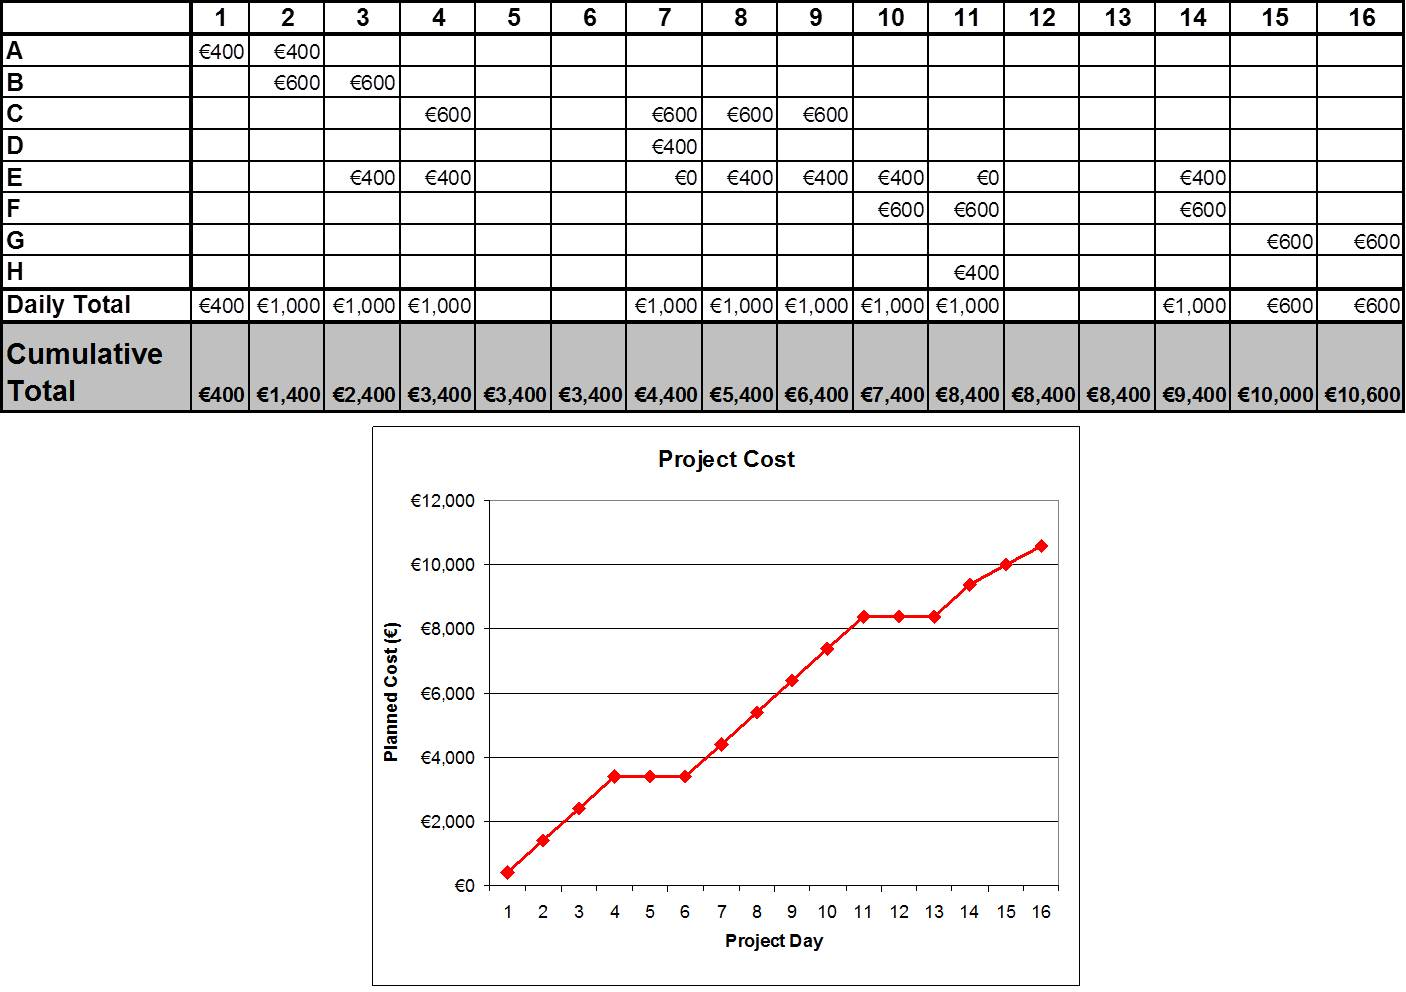
\includegraphics[width = 10cm]{images/useagexl.jpg}
	\label{fig:useagexl}
\end{figure}
\end{frame}
\begin{center}\line(1,0){250}\end{center}






\begin{frame}
\frametitle{}
\begin{figure}
	\centering
		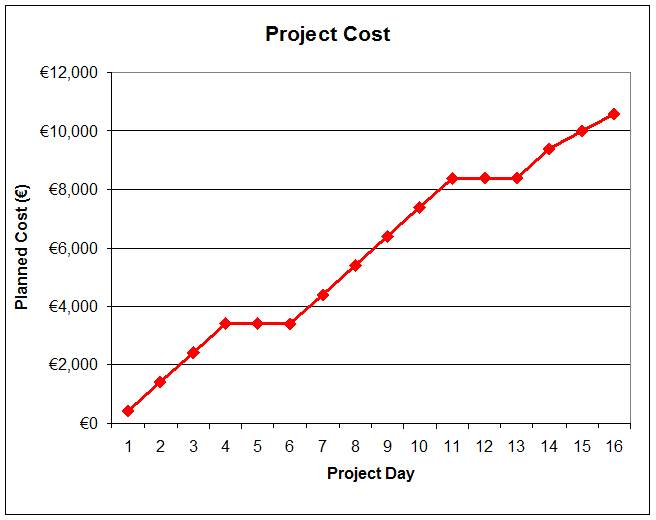
\includegraphics[width = 10cm]{images/costprofile.jpg}
	\label{fig:costprofile}
\end{figure}

\end{frame}
\begin{center}\line(1,0){250}\end{center}






\begin{frame}
\frametitle{Tracked Costs}
\begin{figure}
	\centering
		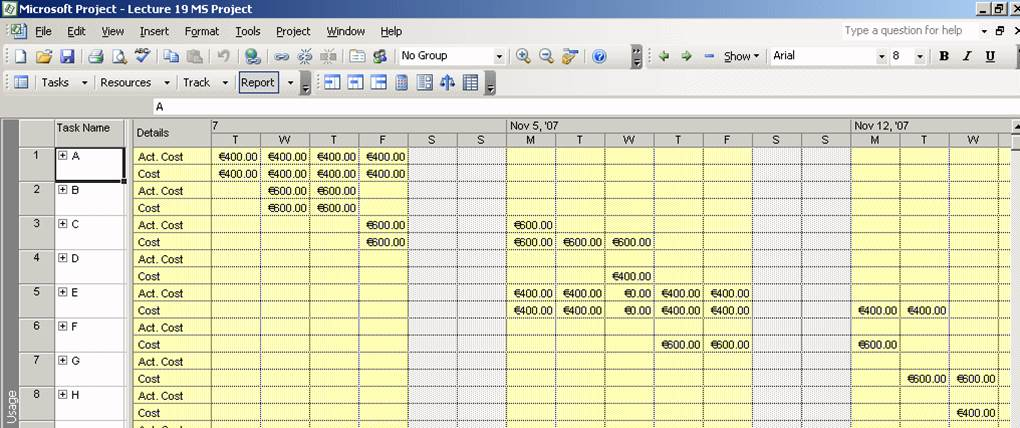
\includegraphics[width = 10cm]{images/costtrack.jpg}
	\label{fig:costtrack}
\end{figure}
\end{frame}
\begin{center}\line(1,0){250}\end{center}






\begin{frame}
\frametitle{Imported to Excel}
\begin{figure}
	\centering
		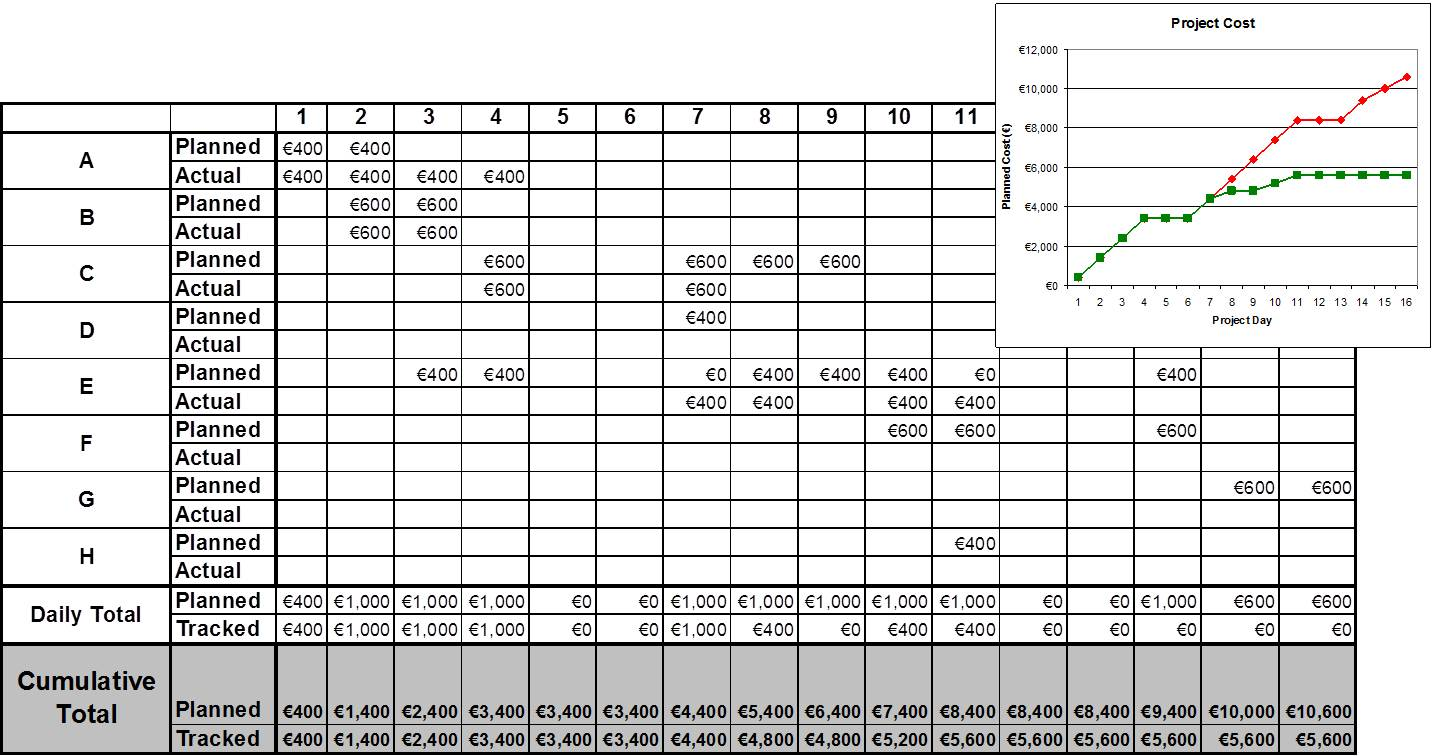
\includegraphics[width = 10cm]{images/costover.jpg}
	\label{fig:costover}
\end{figure}

\end{frame}
\begin{center}\line(1,0){250}\end{center}






\begin{frame}
\frametitle{}
\begin{figure}
	\centering
		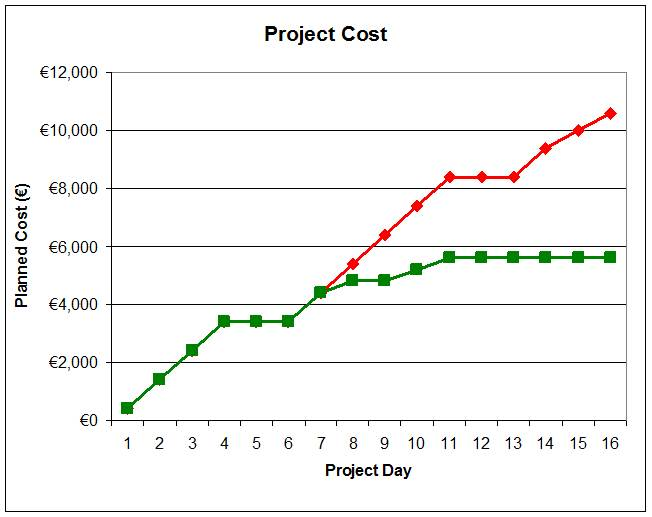
\includegraphics[width = 10cm]{images/costoverlg.jpg}
	\label{fig:costoverlg}
\end{figure}
\end{frame}
\begin{center}\line(1,0){250}\end{center}







\begin{frame}
\frametitle{Cost Estimating \hfill Outputs}
\textbf{Activity Cost Estimates:} Quantitative Estimates of the likely costs of the resources required to complete schedule activities
\begin{itemize}
	\item Labour, Materials, Equipment, Services, Facilities, IT, etc.
	\item May also include Inflation, CPA, contingency, etc.
\end{itemize}
\textbf{Basis of Estimates:} Provide a clear breakdown of how estimates were calculated
\begin{itemize}
	\item Description of schedule activities scope of work
	\item Documentation of basis of estimate
	\item Documentation of assumptions, constraints, etc.
	\item Indication of range and accuracy of estimates
	\begin{itemize}
		\item \euro25,000 $\pm$ \euro2,000
		\item \euro12,000 to \euro14000 
		\item \euro32,000 $\pm$ 10\%
		\item \euro32,000 @ 90\% confidence
	\end{itemize}
\end{itemize}
\end{frame}
\begin{center}\line(1,0){250}\end{center}







\begin{frame}
\frametitle{Cost Estimating \hfill Outputs}
\textbf{Project Document Updates}\\
\begin{itemize}
	\item The process of estimating may highlight specific issues that may not previously been considered.
	\item These 'new' issues may have to be incorporated into the Project Documentation
\end{itemize}
\end{frame}
\begin{center}\line(1,0){250}\end{center}








\begin{frame}
\frametitle{Estimating Pitfalls}
\begin{itemize}
	\item Misinterpretation of Statement of Work
	\item Omissions or Improperly defined Project Scope
	\item Poorly defined or over optimistic project schedule
	\item Inaccurate Work Breakdown Structure (WBS)
	\item Applying improper skill level to tasks
	\item Failure to account for Risk
	\item Failure to account for CPA and Inflation
	\item Failure to use forward pricing rates for overhead, general admin, etc.
	\item Most of these pitfalls are tend not to be recognised until the project is well underway.
\end{itemize}
\end{frame}
\begin{center}\line(1,0){250}\end{center}







\subsection{Cost Budgeting}

\begin{frame}
\frametitle{Cost Budgeting}
\begin{figure}
	\centering
		\includegraphics[width = 10cm]{images/fig7-6.jpg}
	\label{fig:7-6}
\end{figure}Part of the Planning Process Group
\end{frame}
\begin{center}\line(1,0){250}\end{center}






\begin{frame}
\frametitle{Cost Budgeting}
Golden Rule of Budgeting:\\

\begin{center}
\textbf{'If you have the data; USE IT'}
\end{center}

\begin{itemize}
	\item Most Project Management Systems, Accounts Systems, and other software systems will hold data that can be used for budgeting and subsequent cost control processes.
	\item Quantitative Data analysis is not that difficult to perform once you have setup a system that works.
\end{itemize}
\end{frame}
\begin{center}\line(1,0){250}\end{center}






\begin{frame}
\frametitle{Sigmoid curve}
Mathematical formula for S-curves: \\

\[
f(x) = \frac{1}{1+e^{-t}}
\]

\[
f(x) = \frac{1}{\lambda+\beta e^{-\alpha t}}
\]


%\begin{tikzpicture}[domain=0:4, yscale=4] 
%    \def\cumulative{\x,{1/(1 + exp((0-\x))}}
%    \draw[very thin,color=gray, step=0.25] (-6.1,-0.025) grid (5.9,1.1) ;
%    \draw[very thick, ->] (-6.1,0) -- (6,0) node[right] {Project Time} ; 
%    \draw[very thick, ->] (-6,-0.025) -- (-6,1.2) node[above] {\% Budget };
%	\draw[thick,color=red,domain=-6:6] plot (\cumulative) node[right] {$f(x) = \frac{1}{1+e^{-t}}$};
%	\node at (-6.4,0.25) {25\%};
%	\node at (-6.4,0.50) {50\%};
%	\node at (-6.4,0.75) {75\%};
%	\node at (-6.5,1.0) {100\%};
%	\node at (0,-.1){\textbf{Project Time}};
%\end{tikzpicture}

\end{frame}
\begin{center}\line(1,0){250}\end{center}




\begin{frame}
\frametitle{Sigmoid curve}
Mathematical formula for S-curves:
\scalebox{0.7}{
\begin{tikzpicture}[domain=0:4, yscale=4] 
    \def\cumulative{\x,{1/(1 + exp((0-\x)))}}
    \draw[very thin,color=gray, step=0.25] (-6.1,-0.025) grid (5.9,1.1) ;
    \draw[very thick, ->] (-6.1,0) -- (6,0) node[right] {Project Time} ; 
    \draw[very thick, ->] (-6,-0.025) -- (-6,1.2) node[above] {\% Budget };
	\draw[thick,color=red,domain=-6:6] plot (\cumulative) node[right] {$f(x) = \frac{1}{1+e^{-t}}$};
	\node at (-6.4,0.25) {25\%};
	\node at (-6.4,0.50) {50\%};
	\node at (-6.4,0.75) {75\%};
	\node at (-6.5,1.0) {100\%};
	\node at (0,-.1){\textbf{Project Time}};
\end{tikzpicture}
}
\end{frame}
\begin{center}\line(1,0){250}\end{center}







\begin{frame}
\frametitle{Effect of changing $\alpha$}
\scalebox{0.7}{
\begin{tikzpicture}[domain=0:4, yscale=4, xscale=1] 
    \def\cumulative{\x,{1/(1 + exp((0-\x)))}}
    \def\alphaA{\x,{1/(1 + exp((0-\x)*.25))}}
    \def\alphaB{\x,{1/(1 + exp((0-\x)*.5))}}
    \def\alphaC{\x,{1/(1 + exp((0-\x)*2.0))}}
    \def\alphaD{\x,{1/(1 + exp((0-\x)*6))}}
    \draw[very thin,color=gray, step=0.25] (-6.1,-0.025) grid (5.9,1.025) ;
    \draw[very thick, ->] (-6.1,0) -- (6,0) node[right] {Project Time} ; 
    \draw[very thick, ->] (-6,-0.025) -- (-6,1.2) node[above] {\% Budget };
	\draw[thick,color=red,domain=-6:6] plot (\cumulative) node[above] {$f(x) = \frac{1}{1+e^{-t}}$};
	\draw[thick,color=green,domain=-6:6] plot (\alphaA) node[right] {$\alpha = 0.25$};
	\draw[thick,color=blue,domain=-6:6] plot (\alphaB) node[right] {$\alpha = 0.50$};
	\draw[thick,color=cyan,domain=-3:3] plot (\alphaC) node[above] {$\alpha = 2.00$};
	\draw[thick,color=magenta,domain=-1.25:1.25] plot (\alphaD) node[above] {$\alpha = 6.00$};
	\node at (-6.4,0.25) {25\%};
	\node at (-6.4,0.50) {50\%};
	\node at (-6.4,0.75) {75\%};
	\node at (-6.5,1.0) {100\%};
	\node at (0,-.1){\textbf{Effect of Changing $\alpha$}};
\end{tikzpicture}
}
\begin{center}
$\alpha$ controls the slope of the curve 
\end{center}
\end{frame}
\begin{center}\line(1,0){250}\end{center}






\begin{frame}
\frametitle{Effect of Changing $\beta$}
\scalebox{0.7}{
\begin{tikzpicture}[domain=0:4, yscale=4] 
    \def\cumulative{\x,{1/(1 + exp((0-\x)))}}
    \def\betaA{\x,{1/(1 + (0.25*exp(0-\x)))}}
    \def\betaB{\x,{1/(1 + (0.5*exp(0-\x)))}}
    \def\betaC{\x,{1/(1 + (5*exp(0-\x)))}}
    \def\betaD{\x,{1/(1 + (15*exp(0-\x)))}}
    \draw[very thin,color=gray, step=0.25] (-6.1,-0.025) grid (5.9,1.025) ;
    \draw[very thick, ->] (-6.1,0) -- (6,0) node[right] {Project Time} ; 
    \draw[very thick, ->] (-6,-0.025) -- (-6,1.2) node[above] {\% Budget };
	\draw[thick,color=red,domain=-6:6] plot (\cumulative);
	\draw[thick,color=green,domain=-6:4] plot (\betaA) node[above left] {$\beta = 0.05$};
	\draw[thick,color=blue,domain=-6:5] plot (\betaB) node[above] {$\beta = 0.25$};
	\draw[thick,color=cyan,domain=-6:6] plot (\betaC) node[right] {$\beta = 5.00$};
	\draw[thick,color=magenta,domain=-6:6] plot (\betaD) node[below right] {$\beta = 15.00$};
	\node at (-6.4,0.25) {25\%};
	\node at (-6.4,0.50) {50\%};
	\node at (-6.4,0.75) {75\%};
	\node at (-6.5,1.0) {100\%};
	\node at (0,-.1){\textbf{Effect of Changing $\beta$}};
\end{tikzpicture}
}

\begin{center}
$\beta$ controls when the curve will start to increase
\end{center}
\end{frame}
\begin{center}\line(1,0){250}\end{center}







\begin{frame}
\frametitle{Effect of Changing $\lambda$}
\scalebox{0.7}{
\begin{tikzpicture}[domain=0:4, yscale=4, xscale=1] 
    \def\cumulative{\x,{1/(1 + exp((0-\x)))}}
    \def\lambdaA{\x,{1/(0.75 + exp(0-\x))}}
    \def\lambdaB{\x,{1/(1.5 + exp(0-\x))}}
    \def\lambdaC{\x,{1/(2.0 + exp(0-\x))}}
    \def\lambdaD{\x,{1/(3.0 + exp(0-\x))}}
    \draw[very thin,color=gray, step=0.25] (-6.1,-0.025) grid (5.9,1.525) ;
    \draw[very thick, ->] (-6.1,0) -- (6,0) node[right] {Project Time} ; 
    \draw[very thick, ->] (-6,-0.025) -- (-6,1.7) node[above] {\% Budget };
	\draw[thick,color=red,domain=-6:6] plot (\cumulative) node[right] {$f(x) = \frac{1}{1+e^{-t}}$};
	\draw[thick,color=green,domain=-6:6] plot (\lambdaA) node[right] {$\lambda = 0.75$};
	\draw[thick,color=blue,domain=-6:6] plot (\lambdaB) node[right] {$\lambda = 1.50$};
	\draw[thick,color=cyan,domain=-6:6] plot (\lambdaC) node[right] {$\lambda = 2.00$};
	\draw[thick,color=magenta,domain=-6:6] plot (\lambdaD) node[right] {$\lambda = 3.00$};
	\node at (-6.4,0.25) {25\%};
	\node at (-6.4,0.50) {50\%};
	\node at (-6.4,0.75) {75\%};
	\node at (-6.5,1.0) {100\%};
	\node at (-6.5,1.25) {125\%};
	\node at (-6.5,1.50) {150\%};
	\node at (0,-.1){\textbf{Effect of Changing $\lambda$}};
\end{tikzpicture}
}
\begin{center}
$\lambda$ controls the end point; use this to correct to 100\% when $\alpha$ and $\beta$ distort the end point.
\end{center}
\end{frame}
\begin{center}\line(1,0){250}\end{center}






\begin{frame}
\frametitle{}
Consider a \euro4,000,000 contract (ex VAT) that is to be executed over 24 months.  \\
By examination of the cost estimates, the S-curve for project costs has been determined to have an $\alpha$ of 0.6, a $\beta$ of 2.0 and a $\lambda$=0.945\\
\begin{columns}[t]
	\begin{column}[T]{0.7\textwidth}
		
\footnotesize		\textbf{Assumptions}
		\begin{itemize}
			\item Interim Payment Certification and Payment of Invoice takes 1 month
			\item Retention of 5\% for 12 months
		\end{itemize}
		\textbf{Results}
		\begin{itemize}
			\item Based on this model the project will be overdrawn.
			\item Peak overdraft is \euro423k in month 16
			\item Total cost of overdraft is over \euro34,500 at 7\% p.a. at month 24
			\item By month 36 the cost of overdraft is over \euro53k
		\end{itemize}
		
	\end{column}
	\footnotesize
	\begin{column}[T]{0.3\textwidth}
		\begin{figure}
			\centering
				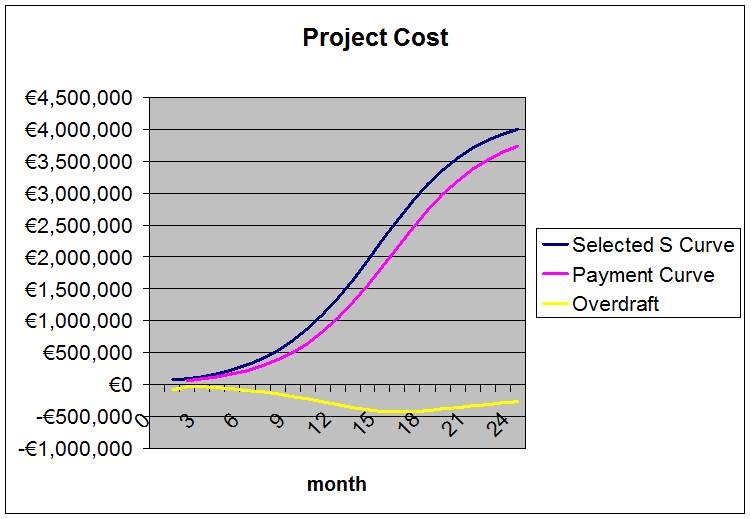
\includegraphics[width=\textwidth]{images/prjcostcurve.jpg}
			\label{fig:prjcostcurve}
		\end{figure}
	\end{column}
\end{columns}
\end{frame}
\begin{center}\line(1,0){250}\end{center}





\begin{frame}
\frametitle{Results}
		\begin{figure}
			\centering
				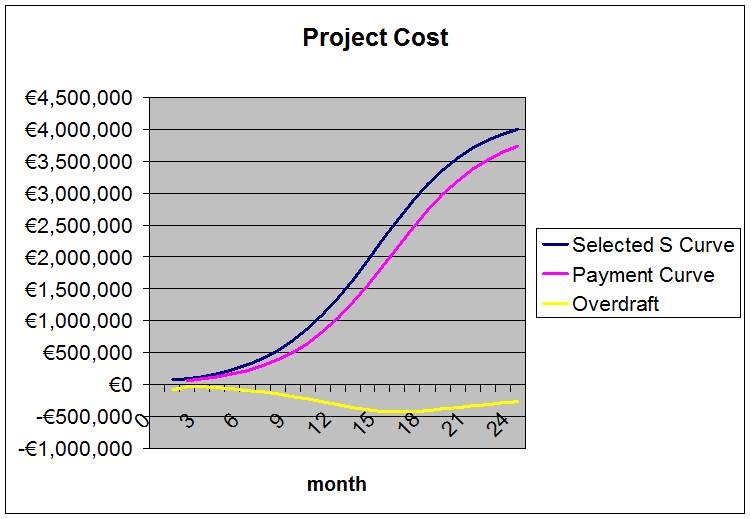
\includegraphics[width = 10cm]{images/prjcostcurve.jpg}
			\label{fig:lgprjcostcurve}
		\end{figure}
\end{frame}
\begin{center}\line(1,0){250}\end{center}






\begin{frame}
\frametitle{Results}
\begin{itemize}
	\item If the project is on a 10\% margin (\euro400k), the cost of the overdraft will reduce the margin to approximately 8.67\%
	\item This calculation assumes that all works claimed for are certified.  If there is delay in certification then the cost of overdraft will be increased, and margins reduced further
\end{itemize}
\end{frame}
\begin{center}\line(1,0){250}\end{center}






\begin{frame}
\frametitle{Effects of Inflation}
\begin{figure}
	\centering
		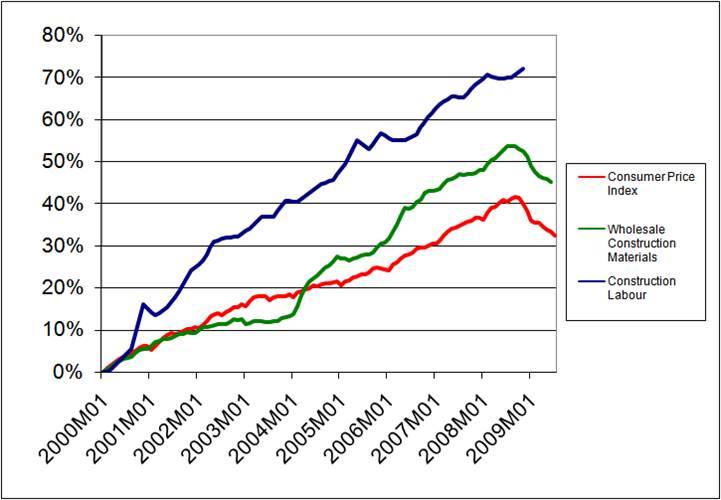
\includegraphics[width = 10cm]{images/deflation.jpg}
	\label{fig:inflation}
\end{figure}
\end{frame}
\begin{center}\line(1,0){250}\end{center}






\begin{frame}
\frametitle{Effects of Inflation}
A tender was submitted at a value of \euro5,000,000 in Jan 2004.\\
\begin{itemize}
	\item The tender was submitted at 15\% margin  
	\item The project is expected to run for 24 months.  
	\item The validity of the tender was 180 days, which was extended by 90 days.  
	\item The CPA clause in the contract was based on the Consumer Price Index (CPI).
\end{itemize}
\end{frame}
\begin{center}\line(1,0){250}\end{center}






\begin{frame}
\frametitle{Inflation Data for Contract Period}
\begin{figure}
	\centering
		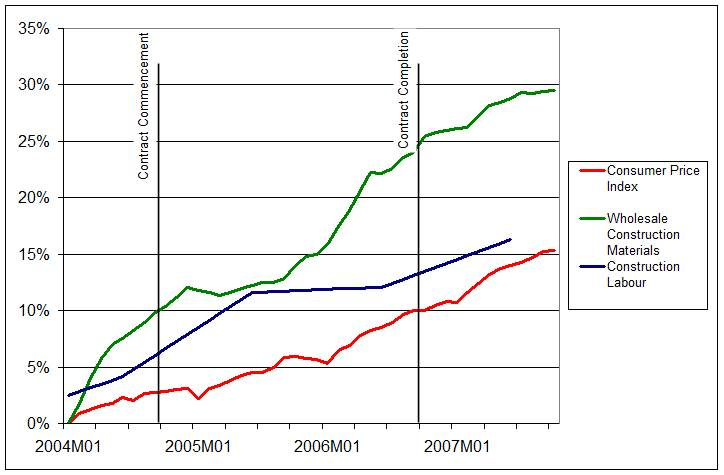
\includegraphics[width = 9cm]{images/infcontract.jpg}
	\label{fig:infcontract}
\end{figure}

\end{frame}
\begin{center}\line(1,0){250}\end{center}






\begin{frame}
\frametitle{}
\textbf{Assumptions and known information}\\
Margin on the contract is \euro750,000
Costs are \euro4,250,000
	\begin{itemize}
		\item Indirect Costs are assumed to be included in labour.
	\end{itemize}
There is an equal split between labour and materials; 50\% materials, 50\% labour
	\begin{itemize}
		\item Material Cost = \euro2,125,000
		\item Labour Cost = \euro2,125,000
	\end{itemize}
\end{frame}
\begin{center}\line(1,0){250}\end{center}







\begin{frame}
\frametitle{}
\textbf{At time of Contract Start}\\
\begin{itemize}
	\item CPI = 2.723\%
	\item Labour Index = 6.044
	\item Material Index = 9.80
\end{itemize}
%
\textbf{Cost Increase to Contractor}\\
\begin{itemize}
	\item \euro2,125,000 $\times$ 1.06044 = \euro2,253,435.00
	\item \euro2,125,000 $\times$ 1.0980 = 	\euro2,333,250.00
	\item			Total	\euro4,586,685.00
\end{itemize}
\textbf{Recoverable via CPA based on CPI}\\
\euro5,000,000 $\times$ 1.02723 = \euro5,136,150\\
\textbf{Loss to Contractor}\\
\euro336,685 - \euro136,150 = \euro200,535
\end{frame}
\begin{center}\line(1,0){250}\end{center}






\begin{frame}
\frametitle{}
\begin{figure}
	\centering
		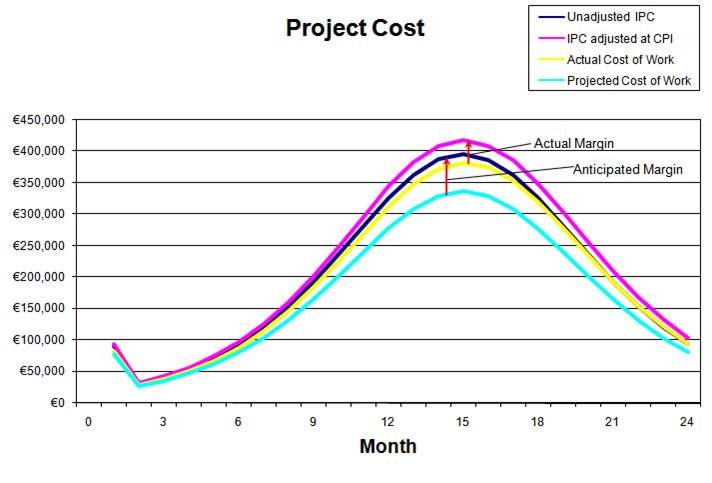
\includegraphics[width = 10cm]{images/projmargin.jpg}
	\label{fig:projmargin}
\end{figure}
\end{frame}
\begin{center}\line(1,0){250}\end{center}






\begin{frame}
\frametitle{}
\begin{figure}
	\centering
		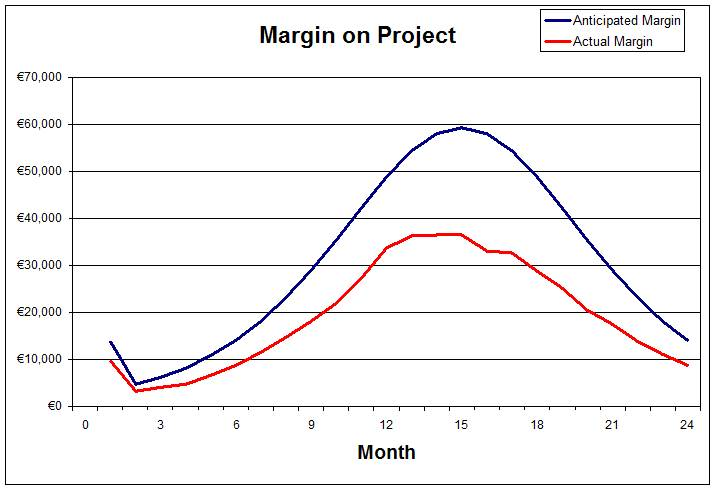
\includegraphics[width = 10cm]{images/margin2.jpg}
	\label{fig:margin2}
\end{figure}

\end{frame}
\begin{center}\line(1,0){250}\end{center}






\begin{frame}
\frametitle{Excel Table - on Moodle}
\begin{figure}
	\centering
		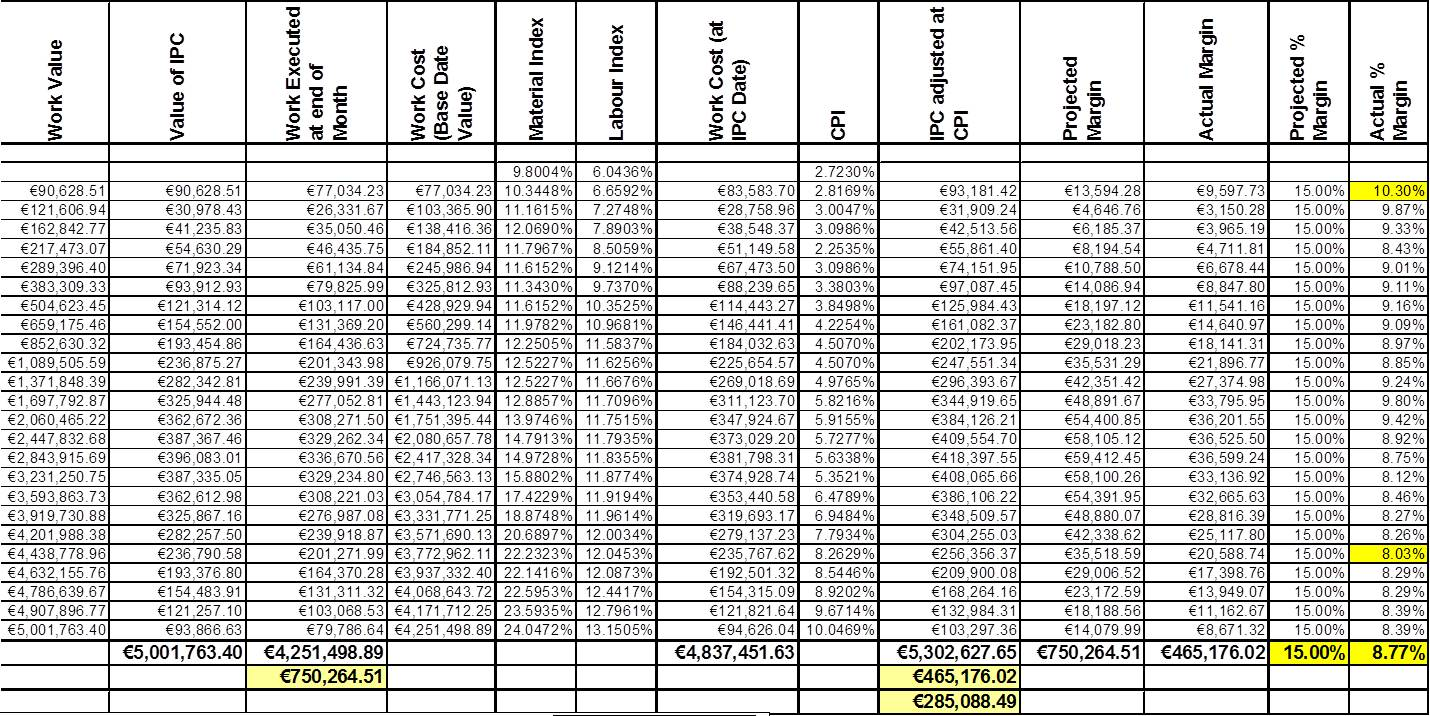
\includegraphics[width = 10cm]{images/rawdata.jpg}
	\label{fig:rawdata}
\end{figure}
\end{frame}
\begin{center}\line(1,0){250}\end{center}






\begin{frame}
\frametitle{Results}
\textbf{Results of Analysis}
\begin{itemize}
	\item Margin Reduced from 15\% to 8.77\%
	\item Margin per month ranged from 10.3\% to 8.03\%
	\item Value of Margin Reduced by approximately \euro285,000 from \euro750,000 to \euro465,176
	\item Margin is reduced the longer the contract continues
\end{itemize}
\begin{itemize}
	\item Failure to perform, or EOT's, likely to have a further negative impact on margin
	\item Analysis does not include 'cost of cash-flow'
\end{itemize}
\end{frame}
\begin{center}\line(1,0){250}\end{center}










\begin{frame}
\frametitle{Cost Budgeting}
\begin{figure}
	\centering
		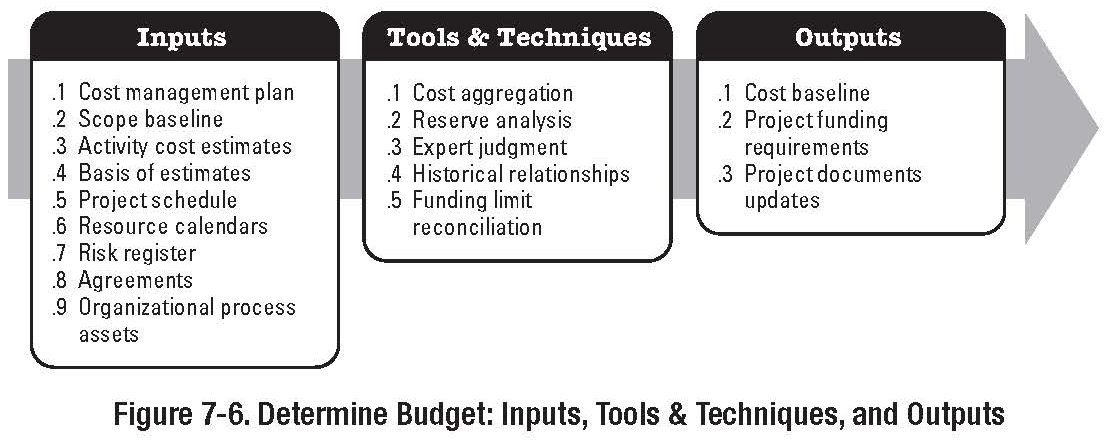
\includegraphics[width = 10cm]{images/Fig7-6.jpg}
	\label{fig:7-6a}
\end{figure}
Part of the Planning Process Group
\end{frame}
\begin{center}\line(1,0){250}\end{center}




\subsection{Deflation}

\begin{frame}
\frametitle{Effects of Deflation}
\begin{figure}
	\centering
		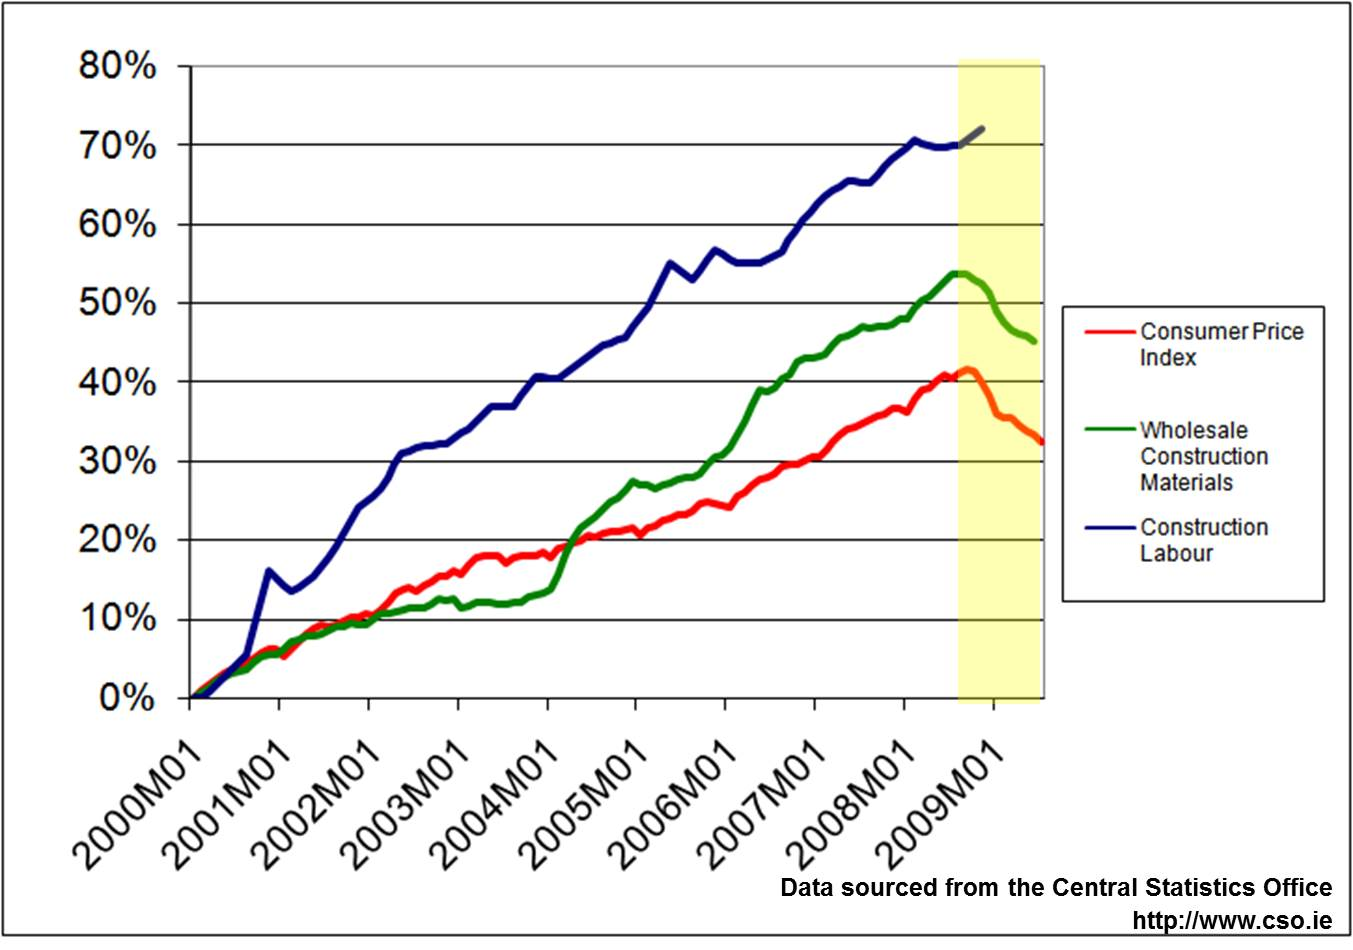
\includegraphics[width = 10cm]{images/deflation2.jpg}
	\label{fig:deflation2}
\end{figure}
\end{frame}
\begin{center}\line(1,0){250}\end{center}







\begin{frame}
\frametitle{Effects of Deflation}

\begin{figure}
	\centering
		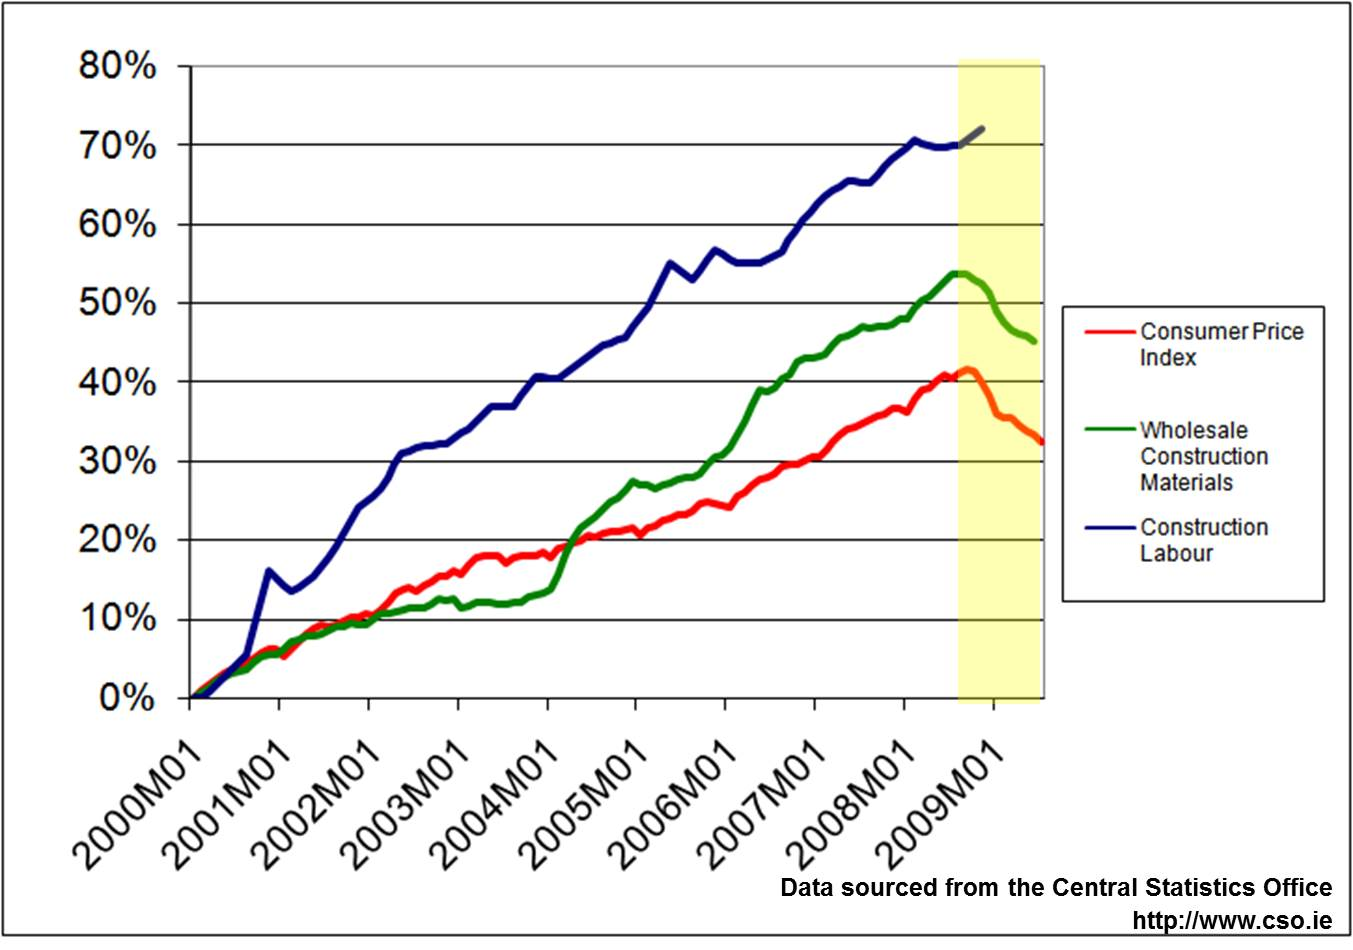
\includegraphics[width = 4cm]{images/deflation2.jpg}
	\label{fig:deflation2a}
\end{figure}

\begin{itemize}
	\item Difficult to predict current impact; economy appears to be on climb out.
	\item Tenders submitted at the peak (Sep 2008) may have been revised downwards during construction phase as part of the CPA clause
	\item If the CPI falls faster than costs, contractors margins will be under threat
\end{itemize}
\end{frame}
\begin{center}\line(1,0){250}\end{center}







\begin{frame}
\frametitle{Effects of Deflation}
\begin{figure}
	\centering
		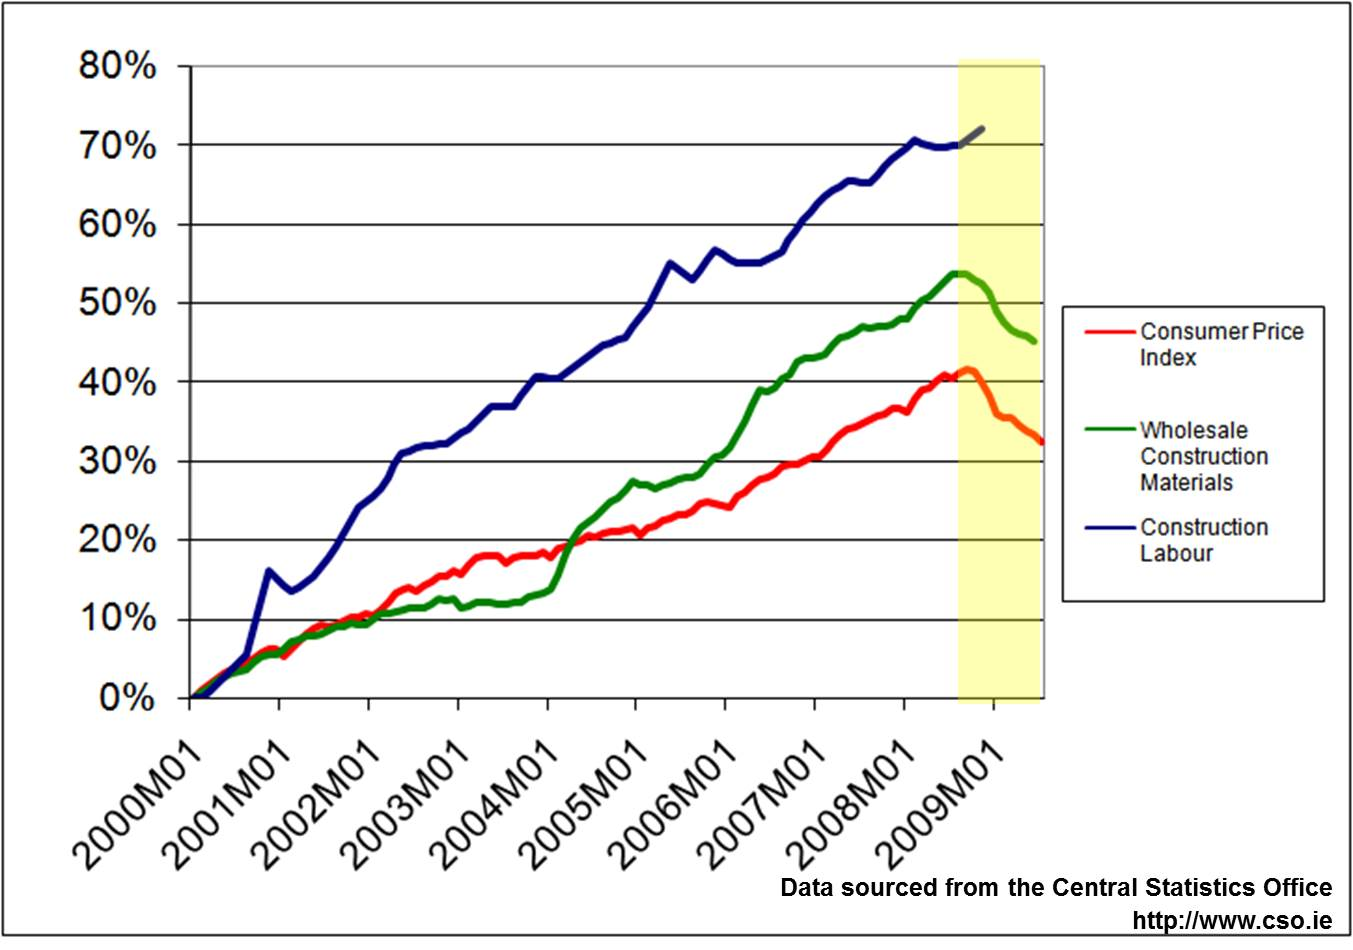
\includegraphics[width = 4cm]{images/deflation2.jpg}
	\label{fig:deflation2b}
\end{figure}
Delays in Interim Payment Certification, combined with retention (5\% to 10\%) leads to significant financial losses.\\
Elapsed time between actually carrying out work and getting payment certification remains critical.\\
\begin{itemize}
	\item In contractors interest to minimise time difference
	\item In clients interest to delay
\end{itemize}
\end{frame}
\begin{center}\line(1,0){250}\end{center}






\begin{frame}
\frametitle{Very Simple Example}
Work carried out during Sept 2008 for  \euro1000.00 including profit
\begin{itemize}
	\item Consumer Price Index: 128
\end{itemize}
Payment approved Dec 2008
\begin{itemize}
	\item Consumer Price Index: 125
	\item Adjustment (125-128) ÷ 128 = -2.3\%
	\item Payment due to contractor \euro977.00
\end{itemize}
Many contractors operate at circa 5\% margin
\begin{itemize}
	\item this margin has effectively been halved.
\end{itemize}
\end{frame}
\begin{center}\line(1,0){250}\end{center}






\begin{frame}
\frametitle{Very Simple Example}
The longer the delay the greater the profit erosion.\\
\begin{figure}
	\centering
		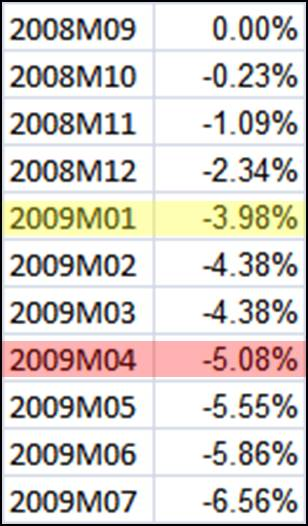
\includegraphics[width = 2cm]{images/proferos.jpg}
	\label{fig:proferos}
\end{figure}
By January 2009 margin is 1.02\%; by April the work is generating a loss.
\end{frame}
\begin{center}\line(1,0){250}\end{center}







\subsection{Contract Examples}

\begin{frame}
\frametitle{}



\begin{figure}
	\centering
		
\includegraphics[width = 6cm]{images/contcvr.jpg}
	\label{fig:contcvr}
\end{figure}
\end{frame}
\begin{center}\line(1,0){250}\end{center}






\begin{frame}
\frametitle{}

\begin{figure}
	\centering
		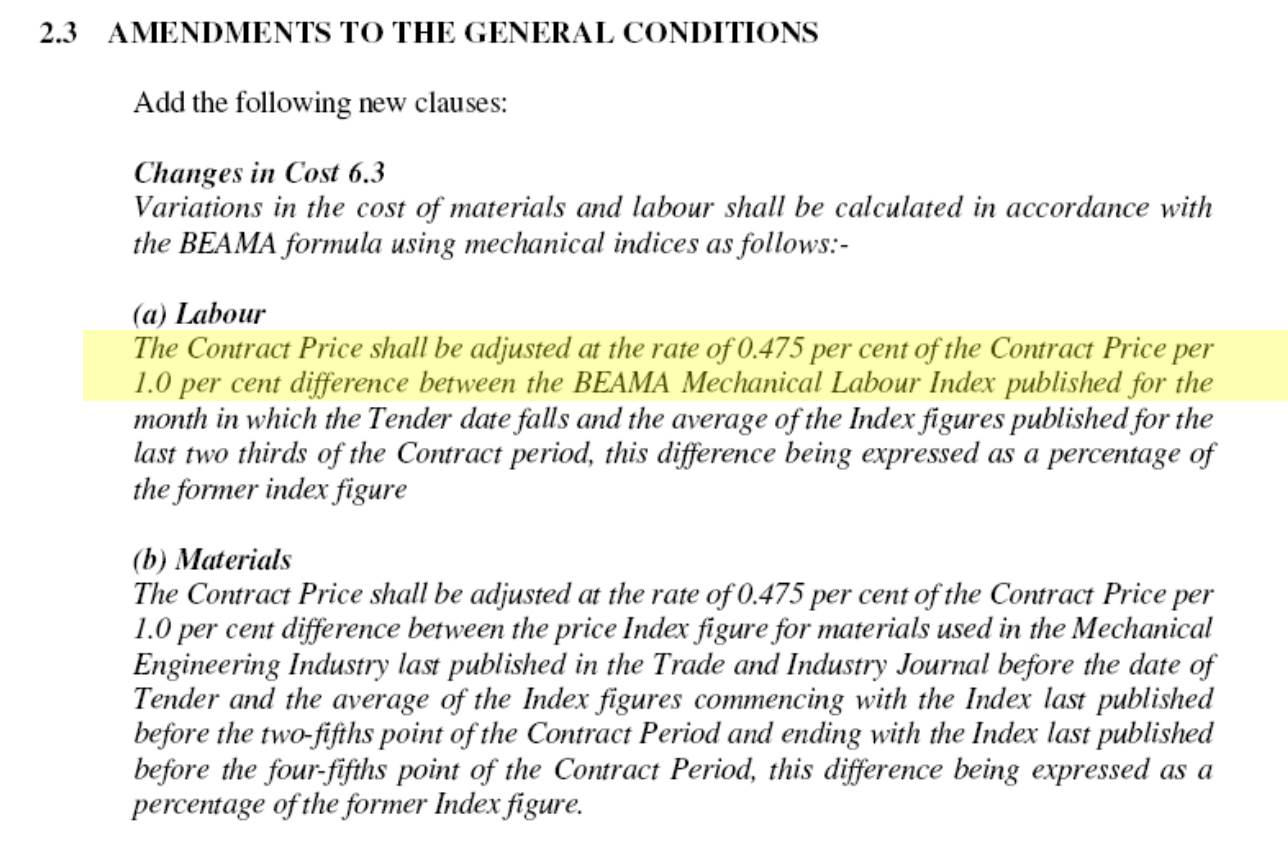
\includegraphics[width = 8cm]{images/conammend.jpg}
	\label{fig:conammend}
\end{figure}

\end{frame}
\begin{center}\line(1,0){250}\end{center}






\begin{frame}
\frametitle{}
\begin{figure}
	\centering
		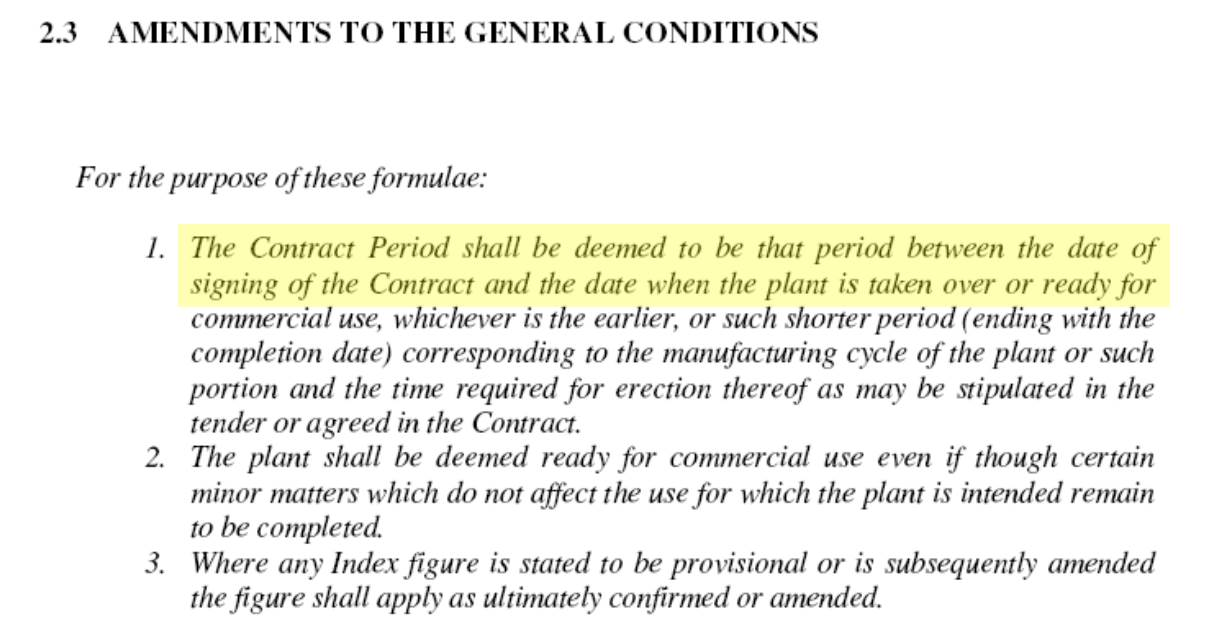
\includegraphics[width = 8cm]{images/conammend2.jpg}
	\label{fig:conammend2}
\end{figure}
On the ITT's for the tender:
\begin{figure}
	\centering
		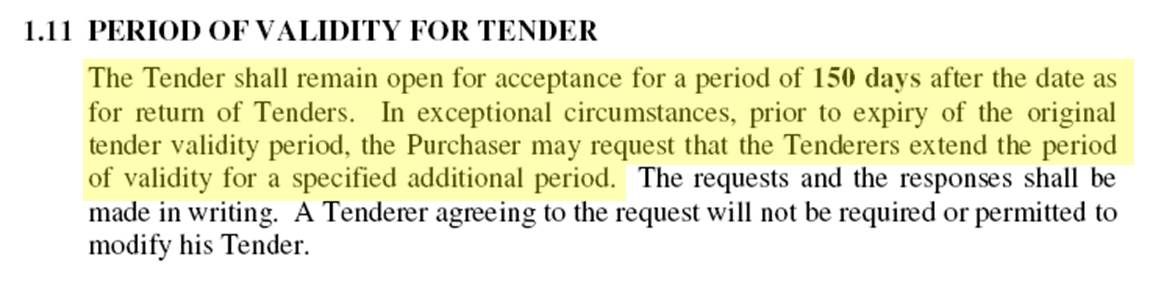
\includegraphics[width = 8cm]{images/convalid.jpg}
	\label{fig:convalid}
\end{figure}
\end{frame}
\begin{center}\line(1,0){250}\end{center}






\begin{frame}
\frametitle{New Gov Contracts}
The new government contracts do not have a Contract Price Adjustment (CPA) Clause.  As a result, the risk of inflation has been passed to the contractor.  \textit{Clause 4.9.3 Civil Engineering Works Designed by the Employer}.
\begin{itemize}
	\item \textbf{Contractors need to learn how to price inflation risk}
\end{itemize}
\end{frame}
\begin{center}\line(1,0){250}\end{center}







\begin{frame}
\frametitle{}
More profit erosion…...
\begin{figure}
 	\centering
 		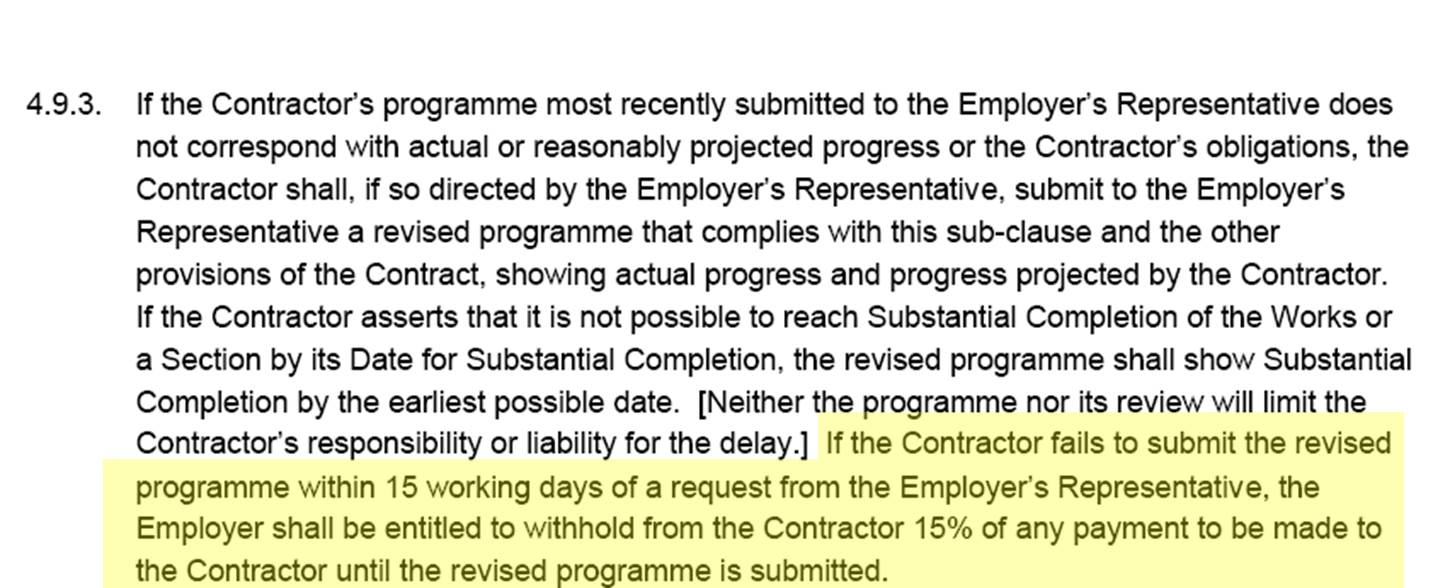
\includegraphics[width = 9cm]{images/dofsch.jpg}
 	\label{fig:dofsch}
 \end{figure}
\end{frame}
\begin{center}\line(1,0){250}\end{center}







\begin{frame}
\frametitle{}
\begin{figure}
	\centering
		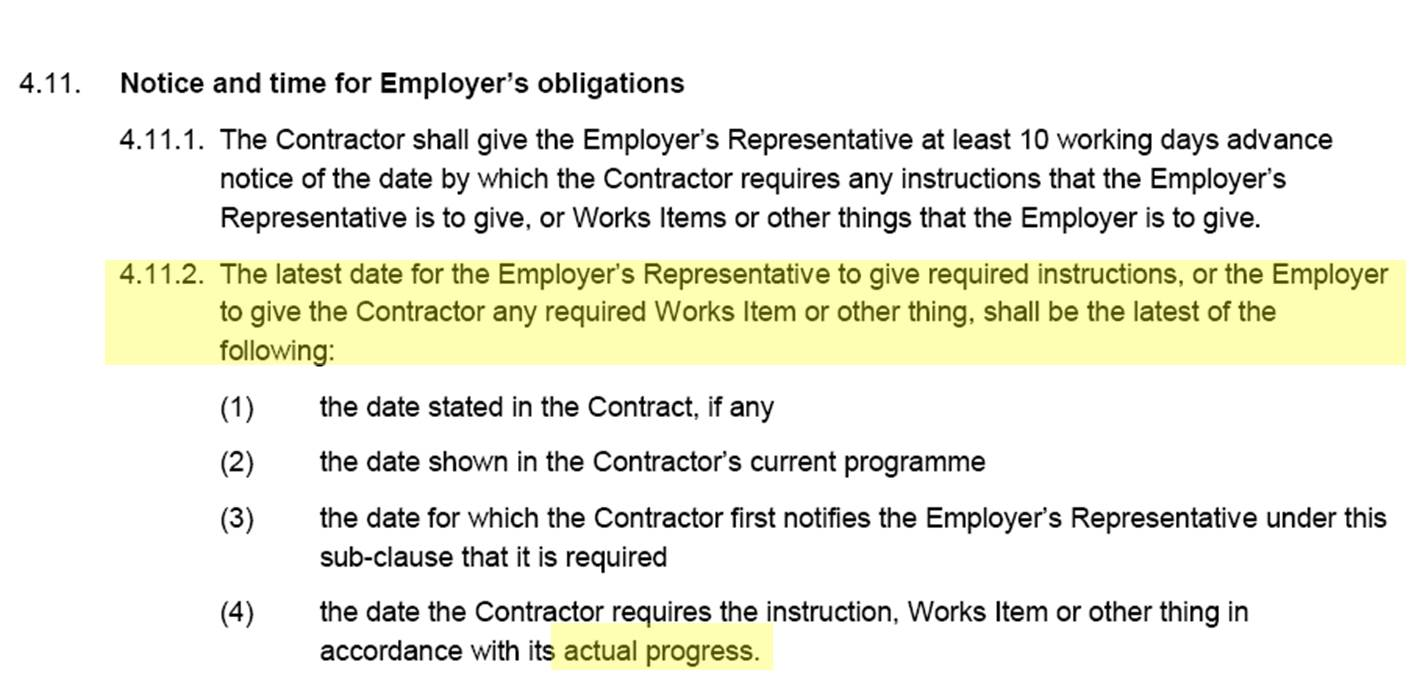
\includegraphics[width = 9cm]{images/dofsch2.jpg}
	\label{fig:dofsch2}
\end{figure}

\textbf{Latest of} \ldots  \textbf{What about planning?}
\begin{itemize}
	\item 'actual progress' may work in contractors favour if 'actual' is taken to include administration time.
\end{itemize}
 
\end{frame}
\begin{center}\line(1,0){250}\end{center}






\begin{frame}
\frametitle{EoT Treatment in Gov Contracts}
\begin{figure}
	\centering
		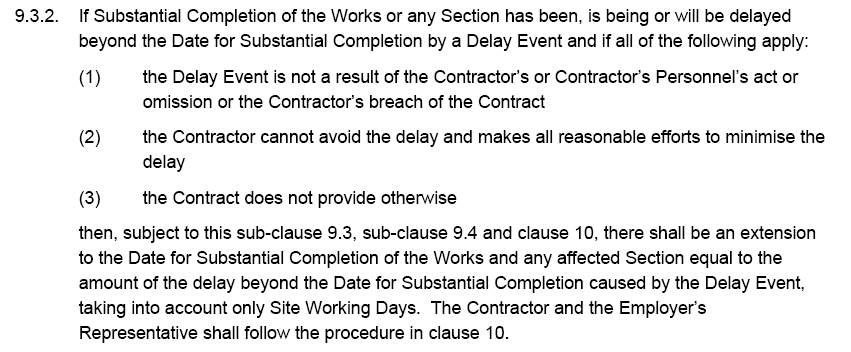
\includegraphics[width = 10cm]{images/delayevt.jpg}
	\label{fig:delayevt}
\end{figure}
\end{frame}
\begin{center}\line(1,0){250}\end{center}






\begin{frame}
\frametitle{EoT Treatment in Gov Contracts}
\begin{figure}
	\centering
		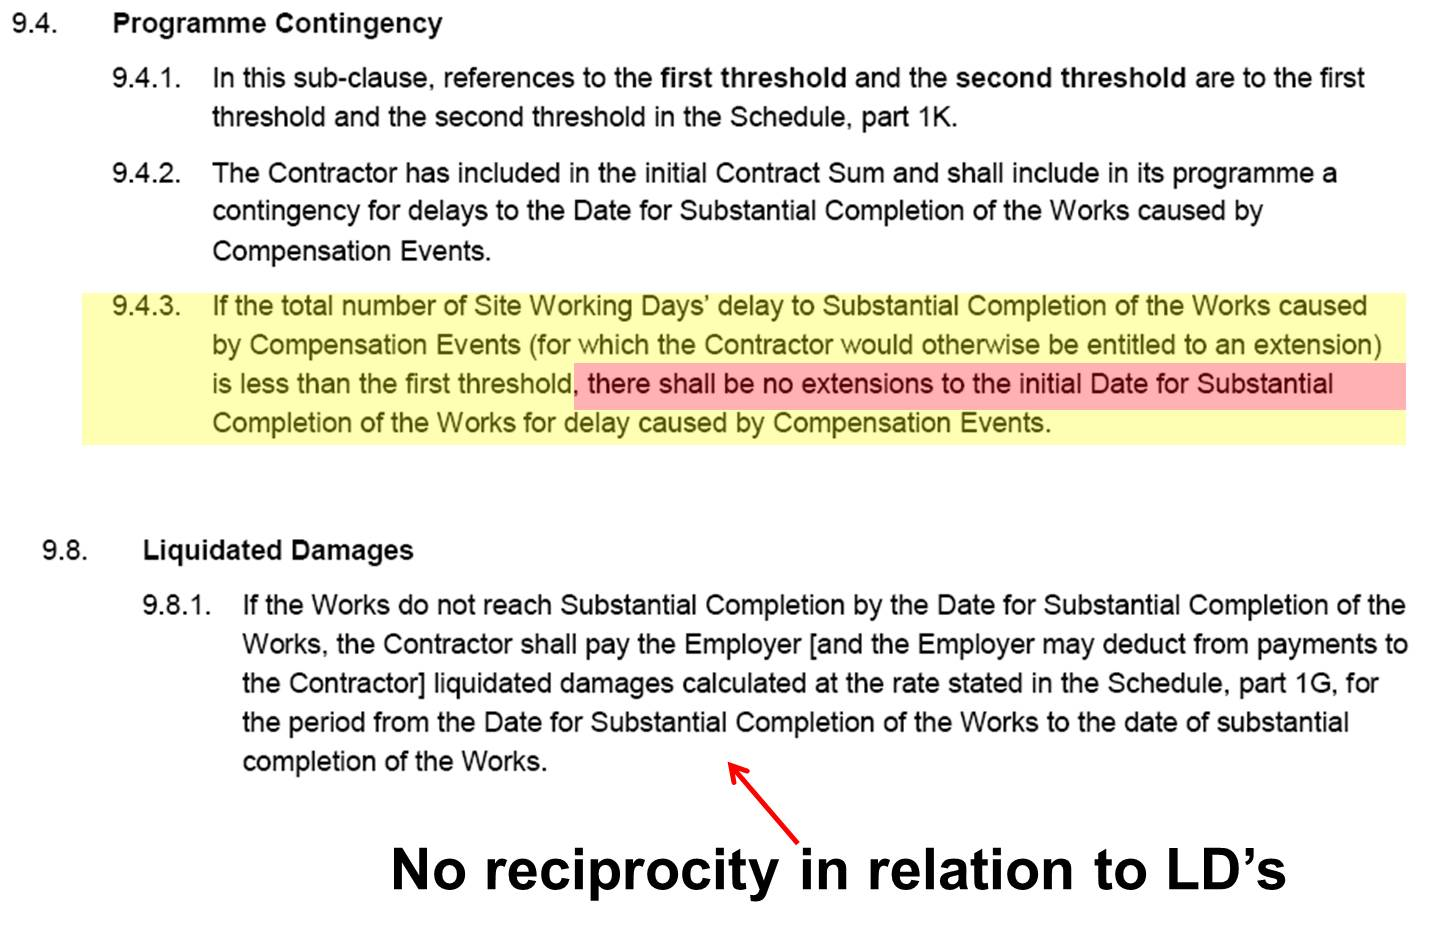
\includegraphics[width = 8cm]{images/eotDOF.jpg}
	\label{fig:eotDOF}
\end{figure}
\end{frame}
\begin{center}\line(1,0){250}\end{center}






\begin{frame}
\frametitle{EoT Treatment in Gov Contracts}
\begin{figure}
	\centering
		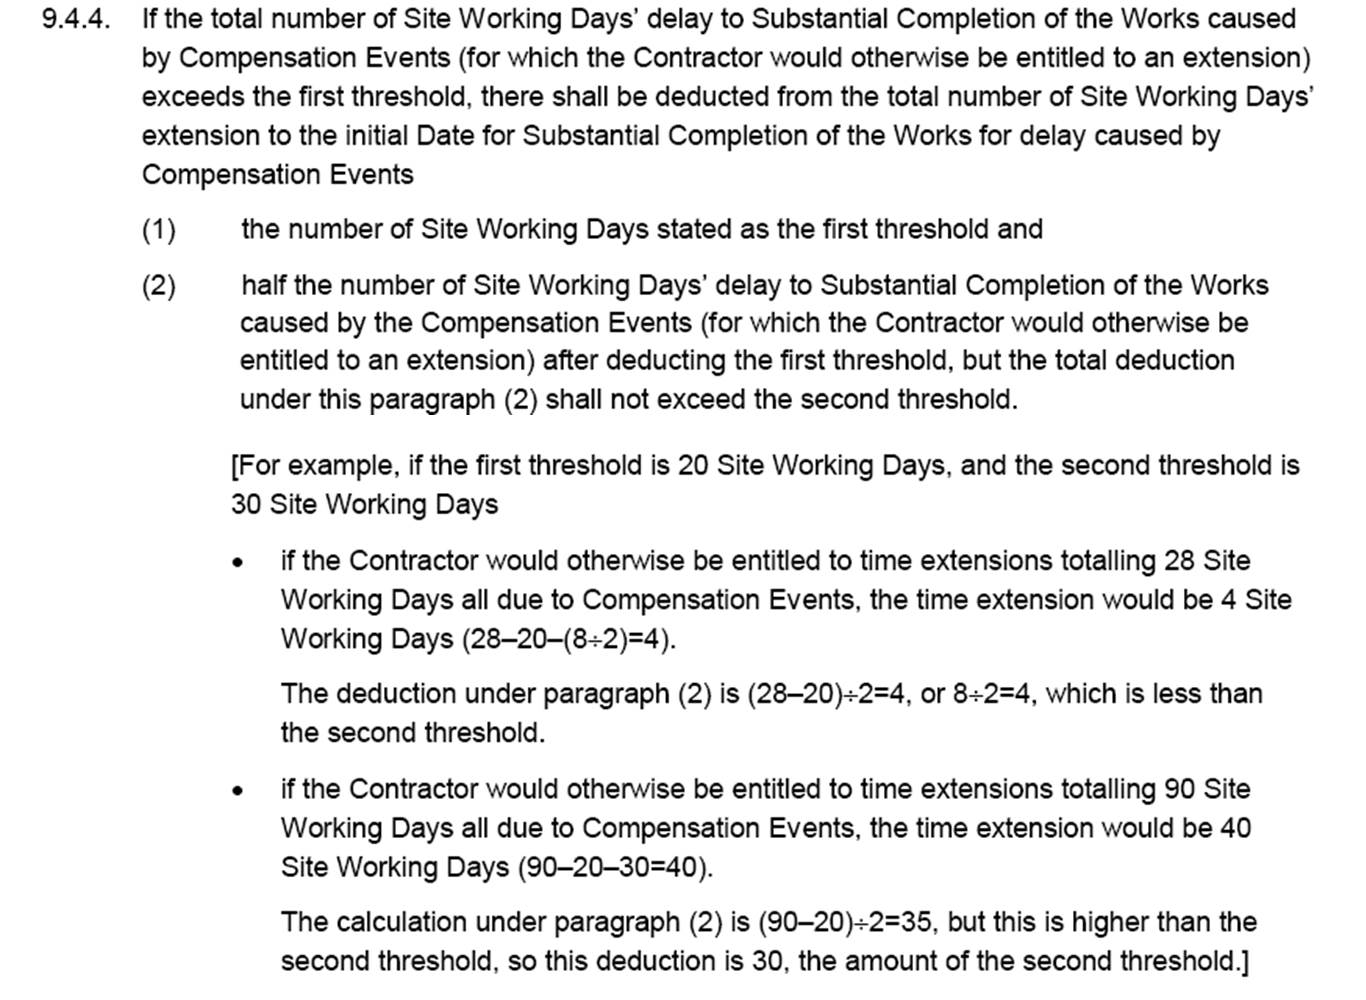
\includegraphics[width = 9cm]{images/eotDOF2.jpg}
	\label{fig:eotDOF2}
\end{figure}
\end{frame}
\begin{center}\line(1,0){250}\end{center}






\begin{frame}
\frametitle{From an Actual Contract}
\begin{figure}
	\centering
		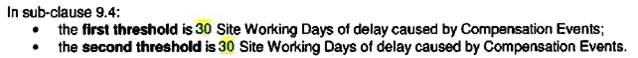
\includegraphics[width = 9cm]{images/cl94.jpg}
	\label{fig:cl94}
\end{figure}
\textbf{Note:} Thresholds are the same.\\
also, anything under 30 days will not yield an actual EoT
\begin{figure}
 	\centering
 		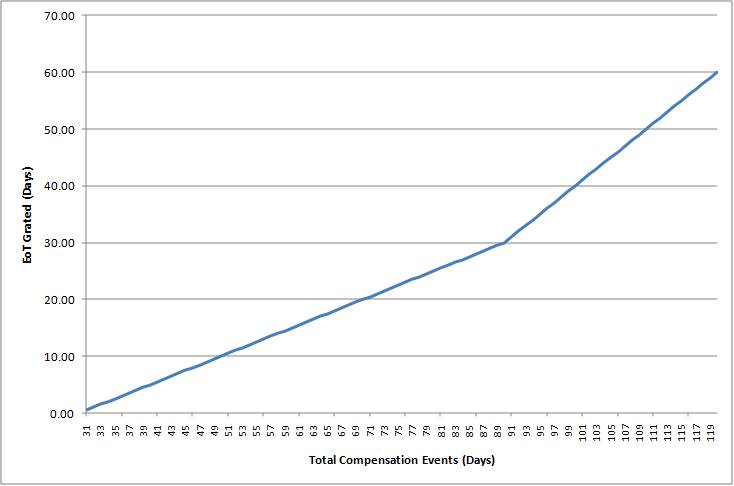
\includegraphics[width = 6cm]{images/cl94grf.jpg}
 	\label{fig:cl94grf}
 \end{figure}
\end{frame}
\begin{center}\line(1,0){250}\end{center}






\begin{frame}
\frametitle{Model of EoT calculation}
\begin{figure}
	\centering
		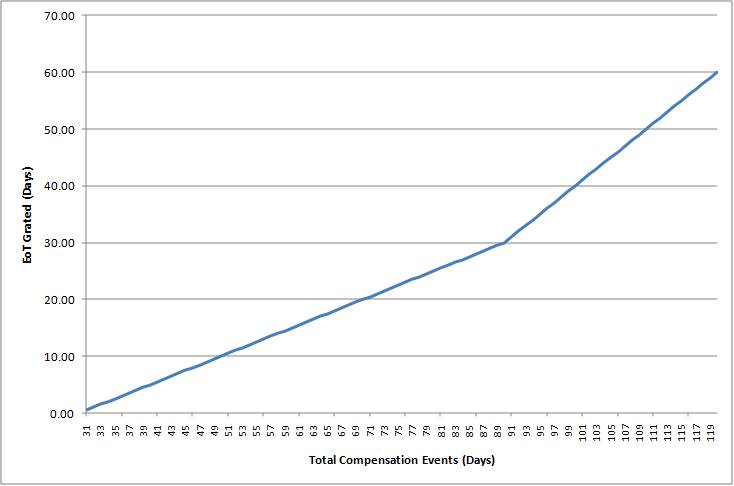
\includegraphics[width = 10cm]{images/cl94grf.jpg}
	\label{fig:cl94grf:dup}
\end{figure}
\end{frame}
\begin{center}\line(1,0){250}\end{center}



\subsection{Determine Budget}


\begin{frame}
\frametitle{Determine Budget}
\begin{figure}
	\centering
		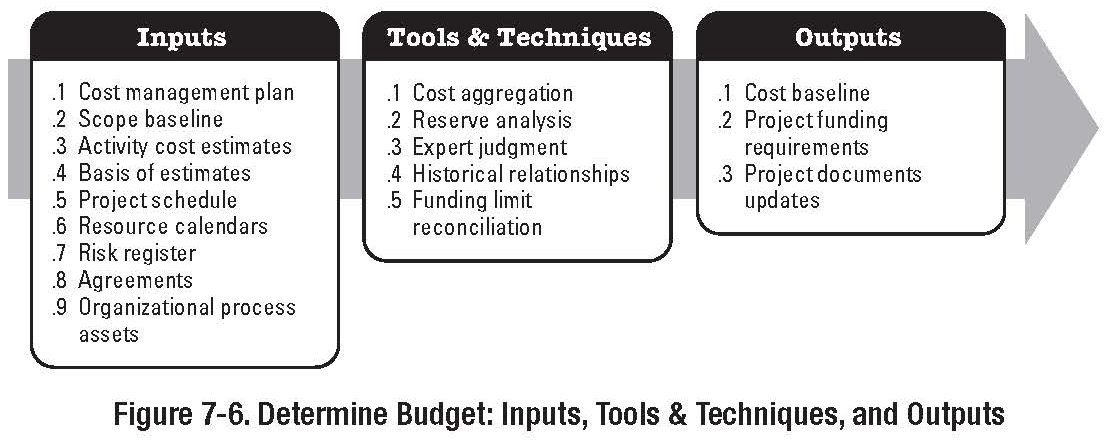
\includegraphics[width = 10cm]{images/Fig7-6.jpg}
	\label{fig:7-6c}
\end{figure}Part of the Planning Process Group
\end{frame}
\begin{center}\line(1,0){250}\end{center}






\begin{frame}
\frametitle{Remember from Previous Lecture}
\begin{figure}
	\centering
		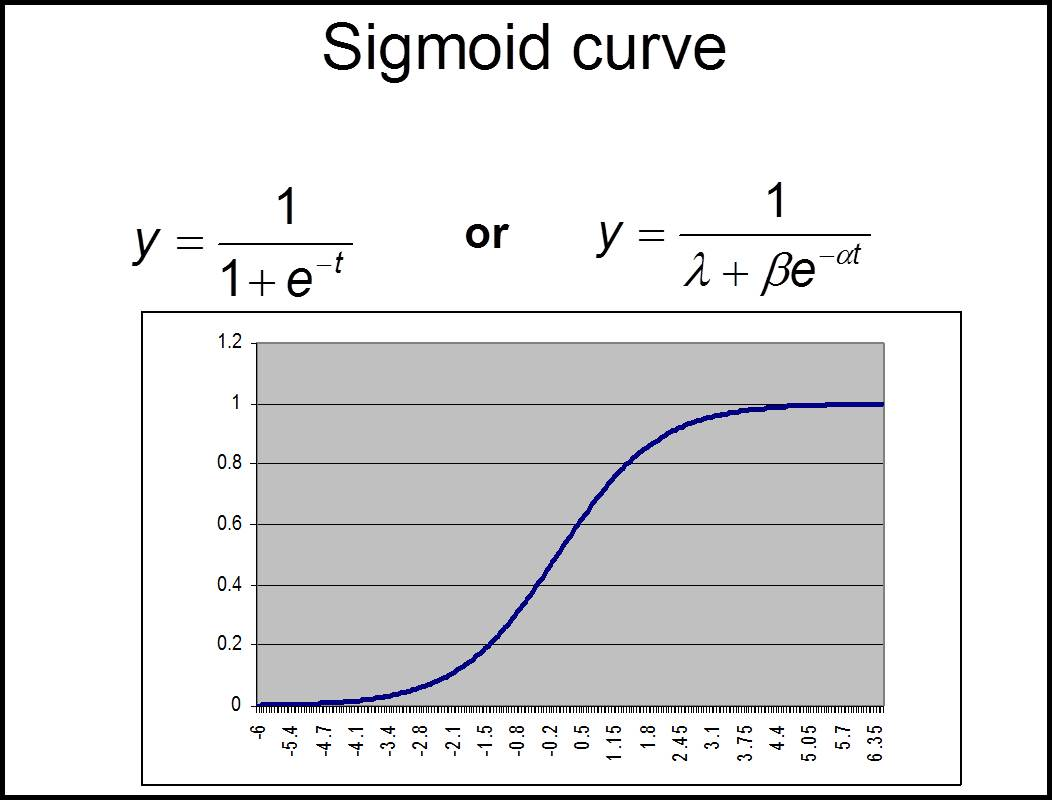
\includegraphics[width = 9cm]{images/sigcurverecap.jpg}
	\label{fig:sigcurverecap}
\end{figure}
\end{frame}
\begin{center}\line(1,0){250}\end{center}






\begin{frame}
\frametitle{Some notes on S-Curve}
\begin{itemize}
	\item S-curves are useful in at the beginning of a project
	\item As time progresses, estimates can be refined, and a more realistic financial model can be developed
	\item Over-reliance on S-curves can create cash-flow difficulties
	\begin{itemize}
		\item What if the $\alpha$, $\beta$, or $\lambda$ are not a good fit to the actual cash flow of the project?
	\end{itemize}
\end{itemize}	
\end{frame}
\begin{center}\line(1,0){250}\end{center}






\begin{frame}
\frametitle{Determine Budget}
\textbf{Inputs}
\begin{itemize}
	\item As per book
\end{itemize}
\textbf{Tools and Techniques}
\begin{itemize}
	\item Cost Aggregation
	\begin{itemize}
		\item Sum of the costs associated with individual work packages and elements from the WBS
	\end{itemize}
	\item Reserve Analysis
	\begin{itemize}
		\item Sum of project cost reserves, such as risk reserve and others
	\end{itemize}
	\item Historical Relationships
	\begin{itemize}
		\item Parametric and/or analogous estimates
		\item Mathematical Models to predict total cost
		\item Refer to book 
		\item\textbf{CAUTION:} models should be treated with care; before use they should be fully understood
	\end{itemize}
\end{itemize}
\end{frame}
\begin{center}\line(1,0){250}\end{center}






\begin{frame}
\frametitle{Determine Budget \hfill\hfill Tools and Techniques }

\textbf{Funding Limit Reconciliation}\\
\begin{itemize}
	\item Modification of the project program in order to smooth out the funding requirements of the project.
	\item Needs to be treated with extreme caution by the contractor
	\item Generally beneficial to the client.
		\begin{itemize}
			\item Projects generally have a value to the client, and generate a return on investment.  The shorter the time between paying the contractor and realising a return from the investment, the better it is for the client
			\item Also, loan interest is incurred from 'drawdown'.  If drawdown can be postponed, less loan interest is incurred.
		\end{itemize}
	\item Both parties need to be aware of Contract Price Adjustment (CPA) Clause and effects
\end{itemize}
\end{frame}
\begin{center}\line(1,0){250}\end{center}






\begin{frame}
\frametitle{Determine Budget}
\begin{figure}
	\centering
		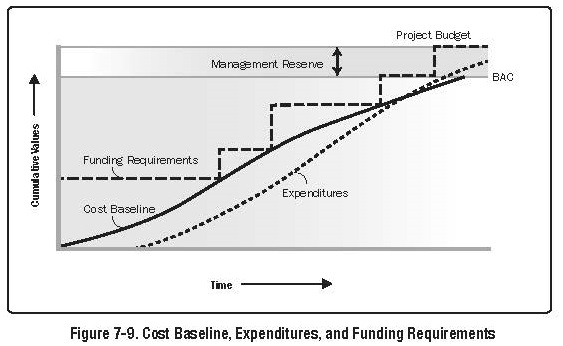
\includegraphics[width = 10cm]{images/Fig7-9.jpg}
	\label{fig:Fig7-9}
\end{figure}

\end{frame}
\begin{center}\line(1,0){250}\end{center}






\begin{frame}
\frametitle{Determine Budget \hfill\hfill Outputs}
\textbf{Cost Performance Baseline}
\begin{itemize}
	\item Time based budget that is used as a basis against which to measure, monitor, and control overall cost performance on the project.
	\item Can be shown as an S-curve
	\item For large construction projects it is normal to include far more detail and track costs against specific cost codes and cost centres.
\end{itemize}
\end{frame}
\begin{center}\line(1,0){250}\end{center}






\begin{frame}
\frametitle{Determine Budget \hfill\hfill Outputs}

\textbf{Project Funding Requirements}
\begin{itemize}
	\item Details the total and periodic funding requirements
	\item Also included a +/- margin for error or changes that may be required
	\item Generally funding requirement are represented by a step function, See Fig 7-9
	\item Contingency reserves are normally spread evenly over the duration of the project.  
\end{itemize}
\end{frame}
\begin{center}\line(1,0){250}\end{center}







\begin{frame}
\frametitle{Determine Budget \hfill\hfill Outputs}
\textbf{Project Document Updates}
\begin{itemize}
	\item Cost Estimates
	\item Risk Register
	\item Project Schedule
\end{itemize}
\end{frame}
\begin{center}\line(1,0){250}\end{center}






\begin{frame}
\frametitle{Control Costs}
\begin{figure}
	\centering
		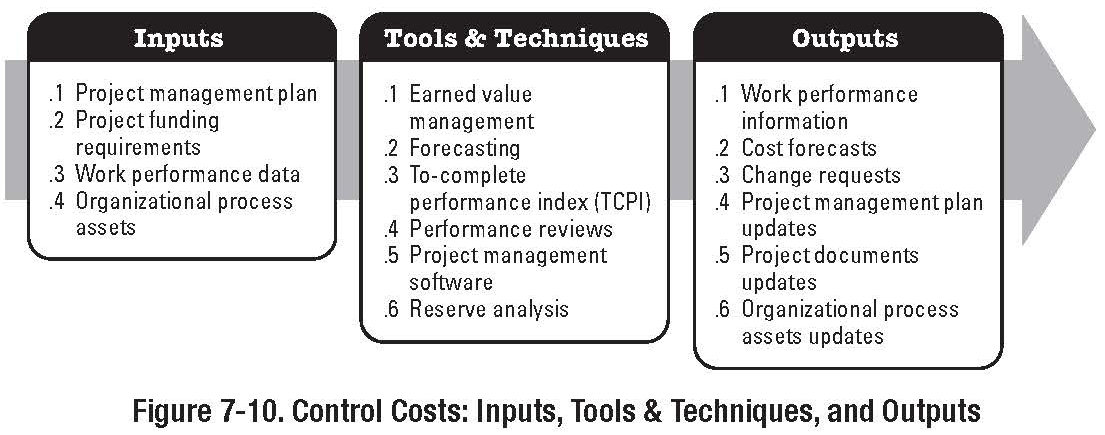
\includegraphics[width = 10cm]{images/Fig7-10.jpg}
	\label{fig:Fig7-10}
\end{figure}
Part of the Monitoring \& Controlling Process Group
\end{frame}
\begin{center}\line(1,0){250}\end{center}







\begin{frame}
\frametitle{Control Costs}
\begin{itemize}
	\item Influencing the factors that create changes to the cost baseline
	\item Ensuring requested changes are agreed upon
	\item Managing the actual changes when and as they occur
	\item Assuring that potential cost overruns do not exceed the authorised funding for the project (total and periodic)
	\item Monitoring cost performance to detect and understand variances from the cost baseline
	\end{itemize}
\end{frame}
\begin{center}\line(1,0){250}\end{center}



\begin{frame}
\frametitle{Control Costs}
\begin{itemize}
	\item Recording all appropriate changes accurately against the cost baseline
	\item Preventing incorrect, inappropriate, or unapproved changes from being included in the reported cost or resource usage
	\item Informing appropriate stakeholders of approved changes
	\item Acting to bring expected cost overruns within acceptable limits (Variations)
\end{itemize}
\end{frame}
\begin{center}\line(1,0){250}\end{center}



\begin{frame}
\frametitle{Control Costs \hfill\hfill Inputs}
\textbf{Cost Baseline and Management Plan}\\
\begin{itemize}
	\item Already covered
\end{itemize}
\textbf{Project Funding Requirements}\\
\begin{itemize}
	\item Already covered
\end{itemize}
\textbf{Performance Reports}\\
\begin{itemize}
	\item  Information and reports on actual cost and resource performance
\end{itemize}
\textbf{Work Performance Information}\\
\begin{itemize}
	\item Deliverables completed and not yet completed
	\item Costs authorised and incurred
	\item Estimates to complete schedule activities
	\item \%age completion of schedule activities
\end{itemize}
\end{frame}
\begin{center}\line(1,0){250}\end{center}







\begin{frame}
\frametitle{Control Costs \hfill Inputs}
\textbf{Organisational Process Assets}\\
	\begin{itemize}
		\item Cost Control policies, procedures \& guidelines
		\item Cost Control Tools
		\item Monitoring and Reporting Methods
	\end{itemize}
\textbf{Tools and Techniques}\\
	\begin{itemize}
		\item Earned Value Management
		\item Forecasting
		\item To-Complete Performance Index (TCPI)
		\item Performance Reviews
		\item Variance Analysis
		\item PM Software
	\end{itemize}
\end{frame}
\begin{center}\line(1,0){250}\end{center}






\begin{frame}
\frametitle{Control Costs- Key Terms}
\begin{itemize}
	\item Planned Value (PV)
	\item Earned Value (EV)
	\item Actual Cost (AC)
	\item Estimate to Completion (ETC)
	\item Estimate at Completion (EAC)
	\item Cost Variance (CV)
	\item Schedule Variance (SV)
	\item Cost Performance Index (CPI)
	\item Schedule Performance Index (SPI)
\end{itemize}
\end{frame}
\begin{center}\line(1,0){250}\end{center}






\begin{frame}
\frametitle{}
\begin{figure}
	\centering
		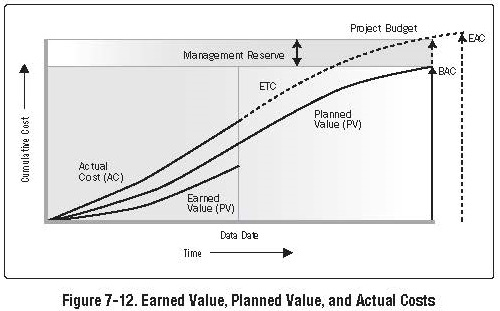
\includegraphics[width = 10cm]{images/Fig7-12.jpg}
	\label{fig:Fig7-12}
\end{figure}

\end{frame}
\begin{center}\line(1,0){250}\end{center}







\begin{frame}
\frametitle{Control Costs- Performance Measurement Analysis}
\textbf{Cost Variance}

\[
	CV = Earned \: Value - Actual\: Cost
\]
\[
	CV = EV - AC
\]

\textbf{Schedule Variance}

\[
	SV = Earned \:Value - Planned \:Value
\]
\[
	SV = EV - PV
\]

\end{frame}
\begin{center}\line(1,0){250}\end{center}






\begin{frame}
\frametitle{Control Costs- Performance Measurement Analysis}

\textbf{Cost Performance Index}\\
Do not confuse with consumer price index..
\[
	CPI = \frac{EV}{AC}
\]
\begin{itemize}
	\item	CPI less than 1.0 indicates cost overrun
	\item	CPI greater than 1.0 indicates cost underrun
\end{itemize}


\textbf{Schedule Performance Index}\\
\[
	SPI = \frac{Earned\: Value}{Planned\: Value} 
\]

\[
	SPI = \frac{EV}{PV}
\]
\end{frame}
\begin{center}\line(1,0){250}\end{center}











\subsection{Earned Value Management}





\begin{frame}
\frametitle{Earned Value Management System}
\begin{itemize}
	\item \textbf{Earned Value} is a management technique that relates resource planning to schedules and technical performance requirements
	\item \textbf{Earned Value Management (EVM)} is a systematic process that uses earned value as the primary tool for integrating cost, schedule, technical performance management and risk management
\end{itemize}
\end{frame}
\begin{center}\line(1,0){250}\end{center}






\begin{frame}
\frametitle{}
For most projects, determination of project progress is extremely difficult without an Earned Value Measurement System (EVMS)\\
Consider a 12 month project: 
\begin{itemize}
	\item value \euro2.5M  
	\item 10 deliverables
\end{itemize}
Report at month 6: 
\begin{itemize}
	\item cost \euro1.75M; 
	\item 4 deliverables complete; 3 deliverables started.
\end{itemize}
Is the project 50\%, 70\% or 40\% complete? 
\end{frame}
\begin{center}\line(1,0){250}\end{center}






\begin{frame}
\frametitle{}
By integrating cost, schedule, technical performance management and risk management, an EVMS will:
\begin{itemize}
	\item Accurately show project status
	\item Assist in the early detection of problems
	\item Assist in the early detection of cost trends
	\item Assist in determining the success of corrective actions
\end{itemize}
EVMS emphasises 'prevention over cure' by identifying and resolving potential issues early.\\
\end{frame}
\begin{center}\line(1,0){250}\end{center}






\begin{frame}
\frametitle{Variance}
\textbf{Cost Variance}
\[
CV = Earned\: Value - Actual\: Cost
\]
\begin{itemize}
	\item Compares deviation from budget
	\item Does not provide a measure of work scheduled against work completed
\end{itemize}
\textbf{Schedule Variance}
\[
SV = Earned\: Value - Planned\: Value
\]
\begin{itemize}
	\item Provides a comparison between planned and actual performance, but does not include costs.
\end{itemize}
\end{frame}
\begin{center}\line(1,0){250}\end{center}






\begin{frame}
\frametitle{Example}
A project was expected to incur costs of \euro100k each week for 4 weeks (PV)\\
Actual expenditure by the end of week 4 was \euro325k (AC), and the Earned Value (EV) was measured at \euro300k.\\
What is the project status?\\
\begin{itemize}
	\item Cost Variance = 300k - 325k = -25k  		(cost overrun)
	\item Schedule Variance = 300k - 400k = -100k 	(behind schedule)
	\item CPI = 300/325 = 0.92 (less than 1.0 therefore cost overrun)
	\item SPI = 300/400 = 0.75 (less than 1.0 therefore behind schedule)
\end{itemize}
\end{frame}
\begin{center}\line(1,0){250}\end{center}






\begin{frame}
\frametitle{CV,SV, CPI and SPI Trends}
Taken in isolation, CV, SV, CPI and SPI have relatively little value; however when graphed over the course of a project trends will emerge that will indicate the project status in a more meaningful way
\end{frame}
\begin{center}\line(1,0){250}\end{center}







\begin{frame}
\frametitle{CV,SV, CPI and SPI Trends}
Consider the following example:
\begin{figure}
	\centering
		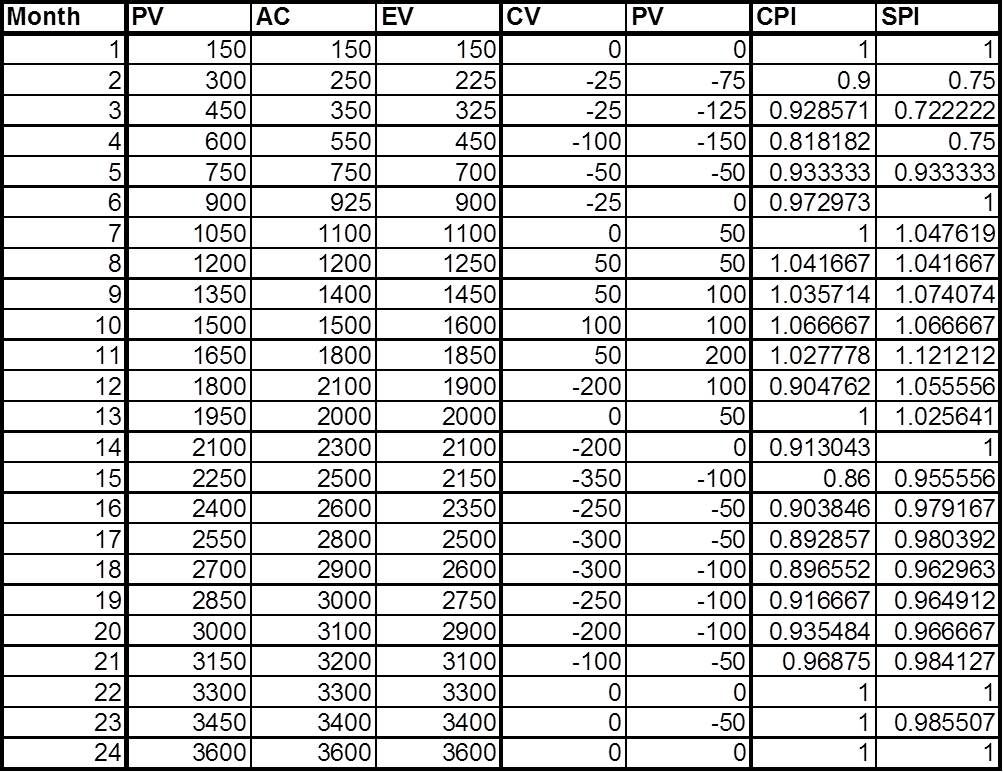
\includegraphics[width = 8cm]{images/trends.jpg}
	\label{fig:trends}
\end{figure}
\end{frame}
\begin{center}\line(1,0){250}\end{center}






\begin{frame}
\frametitle{PV, AC, and EV Trends}
\begin{figure}
	\centering
		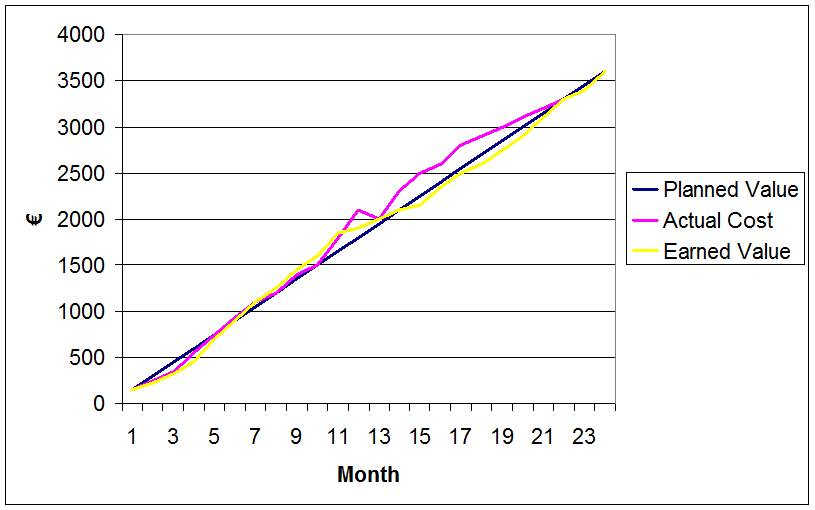
\includegraphics[width = 9cm]{images/trendsgraph.jpg}
	\label{fig:trendsgraph}
\end{figure}
\end{frame}
\begin{center}\line(1,0){250}\end{center}






\begin{frame}
\frametitle{CV and SV Trends}
\begin{figure}
	\centering
		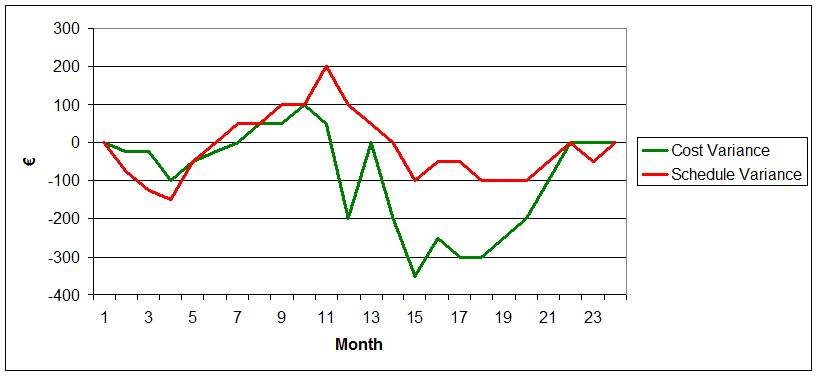
\includegraphics[width = 9cm]{images/cvtrends.jpg}
	\label{fig:cvtrends}
\end{figure}
\end{frame}
\begin{center}\line(1,0){250}\end{center}






\begin{frame}
\frametitle{CPI and SPI Trends}
Favourable or unfavourable trends are very easily identified when the data is graphed.\\
\begin{figure}
	\centering
		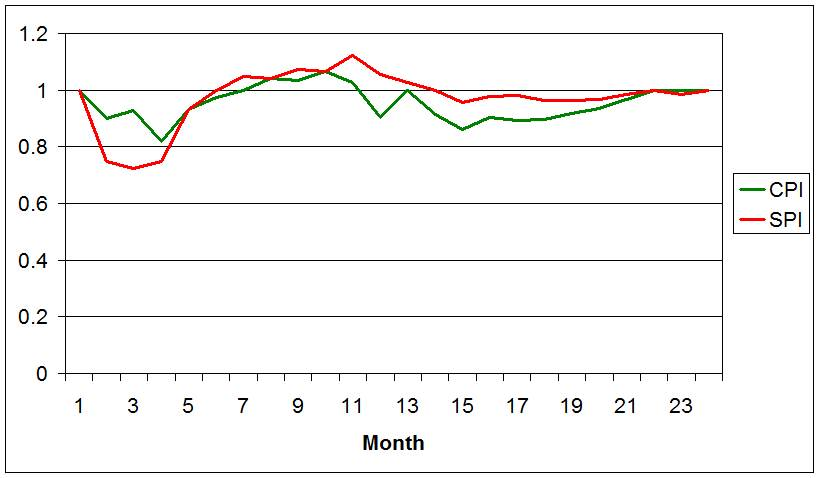
\includegraphics[width = 9cm]{images/cpitrend.jpg}
	\label{fig:cpitrend}
\end{figure}

\end{frame}
\begin{center}\line(1,0){250}\end{center}





\begin{frame}
\frametitle{}
Additional data can also be easily added:
\begin{figure}
	\centering
		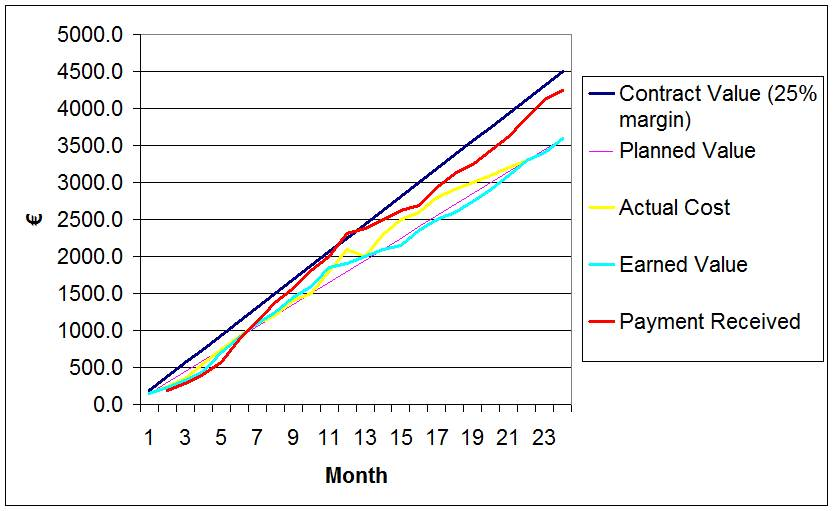
\includegraphics[width = 9cm]{images/alltrends.jpg}
	\label{fig:alltrends}
\end{figure}
\begin{itemize}
	\item In this case Contract Value and Payments Received have been included on a PV,AC and EV graph
\end{itemize}
\end{frame}
\begin{center}\line(1,0){250}\end{center}





\begin{frame}
\frametitle{Variance Analysis}
When analysing variance, a number of key questions need to be considered
\begin{itemize}
	\item What is the problem causing the variance?
	\item What is the impact on time, cost and performance?
	\item What is the impact on other efforts, if any?
	\item What corrective action is planned or underway?
	\item What are the expected results of the corrective action?
\end{itemize}
\end{frame}
\begin{center}\line(1,0){250}\end{center}







\begin{frame}
\frametitle{Work in Progress : '50-50' Rule}
One of the drawbacks of EVM systems is  determining the earned value (EV) of Work in Progress (WIP) where estimating resource input is impractical.  Often the '50-50' rule is used to estimate the earned value of WIP in these cases\\
\textbf{Example:}
\begin{itemize}
	\item Work package cost, \euro15,000
	\item Work package duration, 2 weeks
	\item Cost at end of week 1 is \euro10,000
	\item Therefore \%age completion of the task using the 50-50 rule is:
	\begin{itemize}
		\item 0.5(1/2) + 0.5(10,000/15,000)
		\item	0.25 + 0.333 = .583 or 58.3%
	\end{itemize}
	\item Therefore EV of work package is \euro8,745
\end{itemize}
\end{frame}
\begin{center}\line(1,0){250}\end{center}






\begin{frame}
\frametitle{Estimate to Completion (ETC)}
\begin{itemize}
	\item The baseline budget for a project is often referred to in EVM as the Budget at Completion, or BAC. (see fig. 7-7) 
	\item In general projects rarely follow the baseline budget
	\item Therefore, it is necessary to estimate the remaining cost to complete the project at various intervals as the project progresses
	\item As the project progresses the accuracy of the ETC will be improved.
	\item Revisions of the ETC are carried out at appropriate intervals, such as weekly or monthly.
\end{itemize}
\end{frame}
\begin{center}\line(1,0){250}\end{center}





\begin{frame}
\frametitle{Estimate to Completion (ETC)}
\textbf{ETC can be calculated in a number of ways}
\begin{itemize}
	\item ETC using a new estimate
	\item ETC using the remaining budget
	\item ETC using CPI
\end{itemize}
\textbf{ETC using new estimate}
\begin{itemize}
	\item Normally only used when the original estimate is fundamentally flawed
\end{itemize}
\end{frame}
\begin{center}\line(1,0){250}\end{center}







\begin{frame}
\frametitle{Estimate to Completion (ETC)}
\textbf{ETC using the remaining budget}
\begin{itemize}
	\item Used when variances are seen as atypical, and the project team is confident that further variances are unlikely
\end{itemize}
\[
		ETC_{BGT} = BAC - EV
\]
\textbf{ETC using CPI}
\begin{itemize}
	\item Used when variances to date are seen as being indicative of future variances
\end{itemize}
\[
		ETC_{CPI} = \frac{(BAC - EV)}{CPI}
\]
\end{frame}
\begin{center}\line(1,0){250}\end{center}






\begin{frame}
\frametitle{Estimate at Completion (EAC)}
Another common measure used is the \textbf{Estimate at Completion, EAC}\\
In general the EAC is:
\[
	EAC = AC + ETC
\]	
\begin{itemize}
	\item As the project progresses the accuracy of the EAC will be improved.
	\item Revisions of the EAC are carried out at appropriate intervals, such as weekly or monthly.
\end{itemize}
\end{frame}
\begin{center}\line(1,0){250}\end{center}






\begin{frame}
\frametitle{Estimate at Completion (EAC)}
\textbf{Like ETC, EAC can be calculated in a number of ways}
\begin{itemize}
	\item EAC using a new estimate
	\item EAC using the remaining budget
	\item EAC using CPI
\end{itemize}
\textbf{EAC using new estimate}
\begin{itemize}
	\item Normally only used when the original estimate is fundamentally flawed
\end{itemize}
\[
		EAC = AC + ETC
\]
\end{frame}
\begin{center}\line(1,0){250}\end{center}






\begin{frame}
\frametitle{Estimate at Completion (EAC)}
\textbf{EAC using the remaining budget}
\begin{itemize}
	\item Used when variances are seen as atypical, and the project team is confident that further variances are unlikely
\end{itemize}
\[
		EAC_{BGT} = AC + BAC - EV
\]
\textbf{EAC using CPI}
\begin{itemize}
	\item Used when variances to date are seen as being indicative of future variances
\end{itemize}
\[
		EAC_{CPI} = AC + \frac{(BAC - EV)}{CPI}
\]
\end{frame}
\begin{center}\line(1,0){250}\end{center}






\begin{frame}
\frametitle{Comparison of EAC results}
\begin{figure}
	\centering
		\includegraphics[width = 9cm]{images/compEAC.jpg}
	\label{fig:compEAC}
\end{figure}
\end{frame}
\begin{center}\line(1,0){250}\end{center}






\begin{frame}
\frametitle{Cost Control Problems}
\begin{itemize}
	\item Poor estimating techniques and/or Standards, resulting in unrealistic budgets
	\item Out of sequence start and completion of activities
	\item Inadequate WBS
	\item Lack of Management policy on reporting and control practices
	\item Reducing budgets or bids to be competitive or eliminate 'fat'
	\item Unnoticed or uncontrolled scope change
	\item Poor comparison of actual and planned costs
	\item Unforeseen technical problems
	\item Schedule delays that require overtime or idle time
	\item Unrealistic CPA clause
\end{itemize}
\end{frame}
\begin{center}\line(1,0){250}\end{center}






\begin{frame}
\frametitle{Causes of Cost Overrun}
\textbf{Proposal Phase}
\begin{itemize}
	\item Failure to understand requirements
	\item Unrealistic appraisal of in-house capability
	\item Underestimation of time requirements
\end{itemize}
\textbf{Planning Phase}
\begin{itemize}
	\item Omissions
	\item Inaccurate WBS
	\item Misinterpretation of information
	\item Wrong or inaccurate estimating techniques
	\item Failure to identify and concentrate on major cost elements
	\item Failure to assess and provide for Risk
\end{itemize}
\end{frame}
\begin{center}\line(1,0){250}\end{center}






\begin{frame}
\frametitle{Causes of Cost Overrun}
\textbf{Negotiation Phase}
\begin{itemize}
	\item Forcing a speedy compromise
	\item Procurement ceiling costs
	\item \textit{'Must win the job'} attitude
\end{itemize}
\textbf{Contractual Phase}
\begin{itemize}
	\item Contractual discrepancies
	\item SOW different from RFP requirements
	\item Proposal team different from project team
\end{itemize}
\textbf{Design Phase}
\begin{itemize}
	\item Accepting customer requests without management approval
	\item Problems in customer communications channels and data items
	\item Problems in Design Review meetings
\end{itemize}
\end{frame}
\begin{center}\line(1,0){250}\end{center}






\begin{frame}
\frametitle{Causes of Cost Overrun}
\textbf{Build Phase}
\begin{itemize}
	\item Excessive material cost
	\item Specification that are not acceptable
	\item Disagreement between engineering team, design team, and construction team
\end{itemize}
\end{frame}
\begin{center}\line(1,0){250}\end{center}






\begin{frame}
\frametitle{Cost Control Process \hfill Outputs}
\begin{itemize}
	\item Cost Estimate (Updates)
	\item Cost Baseline (Updates)
	\item Performance Measurements
		\begin{itemize}
			\item CV, SV, CPI, SPI
		\end{itemize}
	\item Forecasted Completion
		\begin{itemize}
			\item ETC, EAC
		\end{itemize}
	\item Requested Changes
	\item Recommended Corrective Actions
	\item Organizational Process Assets (Updates)
	\item Project Management Plan (Updates)
\end{itemize}
\end{frame}
\begin{center}\line(1,0){250}\end{center}







\subsection{EVMS Worked Example}




\begin{frame}
\frametitle{EVMS Worked Example}
\begin{figure}
	\centering
		\includegraphics[width = 5cm]{images/evmsdata.jpg}
	\label{fig:evmsdata}
\end{figure}
The above project has a total planned duration of 35 weeks.  The project is currently at the end of week 12.  Calculate:

\begin{table}
	\centering
		\scalebox{0.6}{
		\begin{tabular}{|l|l|l|l|l|l|}
		\hline
		a)	&PV at week 12				&b)& EV								&c)& CV\\
		d)	&CPI									&e)& SV								&f)& SPI\\
		g)	&ETC based on budget	&h)& ETC based on CPI	&i)& EAC -budget\\
		j)	&ETC based on CPI			&k)& \%age Completion	&l)& \% Budget Spent\\
		m)	&New Project Duration based on SPI\\	
		\hline
		\end{tabular}
			}	
\end{table}
\end{frame}
\begin{center}\line(1,0){250}\end{center}






\begin{frame}
\frametitle{Construct a table}
\begin{figure}
	\centering
		\includegraphics[width = 9cm]{images/evmstable.jpg}
	\label{fig:evmstable}
\end{figure}


\end{frame}
\begin{center}\line(1,0){250}\end{center}






\begin{frame}
\frametitle{Step 2 - Known Information}
\begin{figure}
	\centering
		\includegraphics[width = 9cm]{images/evmknown.jpg}
	\label{fig:evmknown}
\end{figure}

\begin{enumerate}
	\item Activities A, B and E are complete, therefore the Earned Value (EV) of each activity is equal to its Planned Value (PV).
	\item The Planned Values of A and B at the end of week 12 are also equal to their original Planned Values.
	\item Activity E has finished ahead of schedule and requires different treatment.
\end{enumerate}
\end{frame}
\begin{center}\line(1,0){250}\end{center}


\begin{frame}
\frametitle{Step 2 - Known Information}
\begin{figure}
	\centering
		\includegraphics[width = 9cm]{images/evmknown.jpg}
	\label{fig:evmknown}
\end{figure}
The Planned value for activity E at end of Week 12:
\begin{enumerate}
	\item We are assuming that the planned value will accumulate linearly over the task duration.
	\item Note that this is a simplified method; ideally it will be dependent on the task nature.
\end{enumerate}
\[
\frac{8 \: weeks}{9 \: weeks} \times \text{\euro}30,000 = \text{\euro}26,666.67
\]
\end{frame}
\begin{center}\line(1,0){250}\end{center}



\begin{frame}
\frametitle{Step 2 - Known Information}

\begin{figure}
	\centering
		\includegraphics[width = 9cm]{images/evmstep2.jpg}
	\label{fig:evmstep2}
\end{figure}
\begin{itemize}
	\item Sum the Planned Value (PV) Column: This gives the Planned Value for the entire project
	\item Sum the Actual Cost (AC) Column: This give the total spend to date on the project
\end{itemize}
\end{frame}
\begin{center}\line(1,0){250}\end{center}






\begin{frame}
\frametitle{}
\begin{figure}
	\centering
		\includegraphics[width = 9cm]{images/evmstep3.jpg}
	\label{fig:evmstep3}
\end{figure}
For the 50-50 Rule, calculate the percentage of schedule by dividing the work to date by the Planned duration,\\ e.g. Activity C:
\[
\frac{8 \: weeks}{10 \: weeks} = 80.00\% 
\] 
\end{frame}
\begin{center}\line(1,0){250}\end{center}






\begin{frame}
\frametitle{}
\begin{figure}
	\centering
		\includegraphics[width = 9cm]{images/evmstep4.jpg}
	\label{fig:evmstep4}
\end{figure}
Now, calculate the percentage of cost by dividing the Actual Cost (AC) of each activity by its Planned Value (PV),\\ e.g. Activity D:
\[
\frac{\text{\euro}12,500.00}{\text{\euro}25,000.00} = 50.00\% 
\] 
\end{frame}
\begin{center}\line(1,0){250}\end{center}






\begin{frame}
\frametitle{}
\begin{figure}
	\centering
		\includegraphics[width = 9cm]{images/evmstep5.jpg}
	\label{fig:evmstep5}
\end{figure}
Next, calculate the actual percentage completion of each activity using the 50-50 rule; add 50\% of the percentage schedule completion and 50\% of the percentage of cost: \\ e.g. Activity F: 
\begin{align*}
(25.00\% \times 0.5) + (40.00\% \times 0.5) &= 32.50\%\\
12.50\% + 20.00\% &= 32.50\%
\end{align*}
\end{frame}
\begin{center}\line(1,0){250}\end{center}






\begin{frame}
\frametitle{}
\begin{figure}
	\centering
		\includegraphics[width = 9cm]{images/evmstep6.jpg}
	\label{fig:evmstep6}
\end{figure}
There is an alternative calculation that is ONLY applicable if the \%age weightings are 0.5 and 0.5. This is to take an average \\ e.g. Activity F: 
\[
\frac{25.00\% + 40.00\%}{2} = 32.50\% 
\]
\end{frame}
\begin{center}\line(1,0){250}\end{center}







\begin{frame}
\frametitle{}
\begin{figure}
	\centering
		\includegraphics[width = 9cm]{images/evmstep7.jpg}
	\label{fig:evmstep7}
\end{figure}
To calculate the Earned Value (EV) for each activity, multiply the percentage Completion by its Planned Value (PV), \\e.g. Activity C: \\
\[
\text{\euro}15,000.00 \times 75.00\% = \text{\euro}11,250.00 
\]
\end{frame}
\begin{center}\line(1,0){250}\end{center}






\begin{frame}
\frametitle{}
\begin{figure}
	\centering
		\includegraphics[width = 9cm]{images/evmstep8.jpg}
	\label{fig:evmstep8}
\end{figure}
To calculate the Planned Value at this point in time it is necessary to calculate the Planned Values for each activity,\\ e.g Activity G:\\
\[
\text{\euro}15,000.00 \times 37.50\% = \text{\euro}5,625.00 
\]
\end{frame}
\begin{center}\line(1,0){250}\end{center}








\begin{frame}
\frametitle{}
\begin{figure}
	\centering
		\includegraphics[width = 9cm]{images/evmstep9.jpg}
	\label{fig:evmstep9}
\end{figure}
To calculate the Planned Value and Earned Value at this point in time, Sum the individual Earned Values and Planned Values.
\end{frame}
\begin{center}\line(1,0){250}\end{center}







\begin{frame}
\frametitle{}
\begin{figure}
	\centering
		\includegraphics[width = 9cm]{images/evmstep10.jpg}
	\label{fig:evmstep10}
\end{figure}
Summary of information:
\begin{table}
	\centering
		\begin{tabular}{| l | r |}
			\hline
			Budget at Completion (BAC)	&	\euro160,000.00\\
			Actual Cost of Contract to date (AC)	& \euro106,500.00\\
			Earned Value to date (EV)			& \euro96,312.50\\
			Planned Vale to date (PV)			& \euro94,291.67\\
			\hline
		\end{tabular}
\end{table}
\end{frame}
\begin{center}\line(1,0){250}\end{center}




\begin{frame}
\frametitle{Further Calculations}

	\begin{table}
		\centering
	\scalebox{1.0}{	
			\begin{tabular}{| l | r |}
				\hline
				Budget at Completion (BAC)	&	\euro160,000.00\\
				Actual Cost of Contract to date (AC)	& \euro106,500.00\\
				Earned Value to date (EV)			& \euro96,312.50\\
				Planned Vale to date (PV)			& \euro94,291.67\\
				Cost Variance (CV) 						& \textcolor{red}{$-$\euro 10,187.50}\\
				Cost Performance Index (CPI)  &	0.9043\\
				Schedule Variance (SV) 				& \euro 2,020.83\\
				Schedule Performance Index (SPI) & 1.0214\\
				\hline
			\end{tabular}}
	\end{table}

\end{frame}
\begin{center}\line(1,0){250}\end{center}



\begin{frame}
\frametitle{Cost Variance (CV)}
	\begin{table}
		\centering
	\scalebox{0.5}{	
			\begin{tabular}{| l | r |}
				\hline
				Budget at Completion (BAC)	&	\euro160,000.00\\
				Actual Cost of Contract to date (AC)	& \euro106,500.00\\
				Earned Value to date (EV)			& \euro96,312.50\\
				Planned Vale to date (PV)			& \euro94,291.67\\
				Cost Variance (CV) 						& \textcolor{red}{$-$\euro 10,187.50}\\
				Cost Performance Index (CPI)  &	0.9043\\
				Schedule Variance (SV) 				& \euro 2,020.83\\
				Schedule Performance Index (SPI) & 1.0214\\
				\hline
			\end{tabular}}
	\end{table}
\begin{block}{Cost Variance equals the Earned Value less Actual Costs to date}
\begin{equation*}
	\begin{split}
		CV & = EV - AC\\
		CV & = \text{\euro}96,312.50 - \text{\euro}106,500.00\\
		CV & = \text{\euro}-10,187.50
	\end{split}
\end{equation*}
\end{block}
\end{frame}
\begin{center}\line(1,0){250}\end{center}


\begin{frame}
\frametitle{Cost Performance Index (CPI)}
	\begin{table}
		\centering
	\scalebox{0.5}{	
			\begin{tabular}{| l | r |}
				\hline
				Budget at Completion (BAC)	&	\euro160,000.00\\
				Actual Cost of Contract to date (AC)	& \euro106,500.00\\
				Earned Value to date (EV)			& \euro96,312.50\\
				Planned Vale to date (PV)			& \euro94,291.67\\
				Cost Variance (CV) 						& \textcolor{red}{$-$\euro 10,187.50}\\
				Cost Performance Index (CPI)  &	0.9043\\
				Schedule Variance (SV) 				& \euro 2,020.83\\
				Schedule Performance Index (SPI) & 1.0214\\
				\hline
			\end{tabular}}
	\end{table}
\begin{block}{Cost Performance Index equals the Earned Value divided by Actual Costs to date}
\begin{equation*}
	\begin{split}
		CPI & = \frac{EV}{AC} = \frac{\text{\euro}96,312.50}{\text{\euro}106,500.00}\\
		CPI & = 0.9043
	\end{split}
\end{equation*}
\end{block}
\end{frame}
\begin{center}\line(1,0){250}\end{center}






\begin{frame}
\frametitle{Schedule Variance (SV)}
	\begin{table}
		\centering
	\scalebox{0.5}{	
			\begin{tabular}{| l | r |}
				\hline
				Budget at Completion (BAC)	&	\euro160,000.00\\
				Actual Cost of Contract to date (AC)	& \euro106,500.00\\
				Earned Value to date (EV)			& \euro96,312.50\\
				Planned Vale to date (PV)			& \euro94,291.67\\
				Cost Variance (CV) 						& \textcolor{red}{$-$\euro 10,187.50}\\
				Cost Performance Index (CPI)  &	0.9043\\
				Schedule Variance (SV) 				& \euro 2,020.83\\
				Schedule Performance Index (SPI) & 1.0214\\
				\hline
			\end{tabular}}
	\end{table}
\begin{block}{Schedule Variance equals the Earned Value less Planned Value to date}
\begin{equation*}
	\begin{split}
		SV & = EV - PV\\
		SV & = \text{\euro}96,312.50 - \text{\euro}94,291.67\\
		SV & = \text{\euro}2,020.83
	\end{split}
\end{equation*}
\end{block}

\end{frame}
\begin{center}\line(1,0){250}\end{center}


\begin{frame}
\frametitle{Schedule Performance Index (SPI)}
	\begin{table}
		\centering
	\scalebox{0.5}{	
			\begin{tabular}{| l | r |}
				\hline
				Budget at Completion (BAC)	&	\euro160,000.00\\
				Actual Cost of Contract to date (AC)	& \euro106,500.00\\
				Earned Value to date (EV)			& \euro96,312.50\\
				Planned Vale to date (PV)			& \euro94,291.67\\
				Cost Variance (CV) 						& \textcolor{red}{$-$\euro 10,187.50}\\
				Cost Performance Index (CPI)  &	0.9043\\
				Schedule Variance (SV) 				& \euro 2,020.83\\
				Schedule Performance Index (SPI) & 1.0214\\
				\hline
			\end{tabular}}
	\end{table}
\begin{block}{Schedule Performance Index equals the Earned Value divided by Planned Value to date}
\begin{equation*}
	\begin{split}
		SPI & = \frac{EV}{PV} = \frac{\text{\euro}96,312.50}{\text{\euro}94,291.67}\\
		SPI & = 1.0214
	\end{split}
\end{equation*}
\end{block}

\end{frame}
\begin{center}\line(1,0){250}\end{center}










\begin{frame}
\frametitle{Estimate to Completion (ETC) based on Budget}
	\begin{table}
		\centering
	\scalebox{0.5}{	
			\begin{tabular}{| l | r |}
				\hline
				Budget at Completion (BAC)	&	\euro160,000.00\\
				Actual Cost of Contract to date (AC)	& \euro106,500.00\\
				Earned Value to date (EV)			& \euro96,312.50\\
				Planned Vale to date (PV)			& \euro94,291.67\\
				Cost Variance (CV) 						& \textcolor{red}{$-$\euro 10,187.50}\\
				Cost Performance Index (CPI)  &	0.9043\\
				Schedule Variance (SV) 				& \euro 2,020.83\\
				Schedule Performance Index (SPI) & 1.0214\\
				\hline
			\end{tabular}}
	\end{table}
\begin{block}{ETC equals the Budget at Completion less the Earned Value to date}
\begin{equation*}
	\begin{split}
		ETC_{BGT} & = BAC - EV\\
		ETC_{BGT} & = \text{\euro}160,000 - \text{\euro}96,312.50\\
		ETC_{BGT} & = \text{\euro}63,687.50
	\end{split}
\end{equation*}
\end{block}


\end{frame}
\begin{center}\line(1,0){250}\end{center}






\begin{frame}
\frametitle{Estimate to Completion (ETC) based on CPI}
	\begin{table}
		\centering
	\scalebox{0.5}{	
			\begin{tabular}{| l | r |}
				\hline
				Budget at Completion (BAC)	&	\euro160,000.00\\
				Actual Cost of Contract to date (AC)	& \euro106,500.00\\
				Earned Value to date (EV)			& \euro96,312.50\\
				Planned Vale to date (PV)			& \euro94,291.67\\
				Cost Variance (CV) 						& \textcolor{red}{$-$\euro 10,187.50}\\
				Cost Performance Index (CPI)  &	0.9043\\
				Schedule Variance (SV) 				& \euro 2,020.83\\
				Schedule Performance Index (SPI) & 1.0214\\
				\hline
			\end{tabular}}
	\end{table}
	\begin{block}{Two Methods of Calculation}
		\begin{equation*}
			\begin{split}
			ETC_{CPI} & = \frac{BAC - EV}{CPI} = \frac{ETC_{BGT}}{CPI}\\
			ETC_{CPI} & = \frac{\text{\euro}160,000 - \text{\euro}96,312.50}{0.9043}\\
			ETC_{CPI} & = \text{\euro}70,427.40
			\end{split}
		\end{equation*}
	\end{block}
	
	
	
\end{frame}
\begin{center}\line(1,0){250}\end{center}





\begin{frame}
\frametitle{Estimate at Completion (EAC) based on Budget}
	\begin{table}
		\centering
	\scalebox{0.5}{	
			\begin{tabular}{| l | r |}
				\hline
				Budget at Completion (BAC)	&	\euro160,000.00\\
				Actual Cost of Contract to date (AC)	& \euro106,500.00\\
				Earned Value to date (EV)			& \euro96,312.50\\
				Planned Vale to date (PV)			& \euro94,291.67\\
				Cost Variance (CV) 						& \textcolor{red}{$-$\euro 10,187.50}\\
				Cost Performance Index (CPI)  &	0.9043\\
				Schedule Variance (SV) 				& \euro 2,020.83\\
				Schedule Performance Index (SPI) & 1.0214\\
				\hline
			\end{tabular}}
	\end{table}
	\begin{block}{Two Methods of Calculation}
		\begin{equation*}
			\begin{split}
					EAC_{BGT} & = (BAC - EV) + AC = ETC_{BGT} + AC\\
					EAC_{BGT} & = \text{\euro}63,687.50 + \text{\euro}106,500.00\\
					EAC_{BGT} & = \text{\euro}170,187.50
			\end{split}
		\end{equation*}
	\end{block}	
\end{frame}
\begin{center}\line(1,0){250}\end{center}






\begin{frame}
\frametitle{Estimate at Completion (EAC) based on CPI}
	\begin{table}
		\centering
	\scalebox{0.5}{	
			\begin{tabular}{| l | r |}
				\hline
				Budget at Completion (BAC)	&	\euro160,000.00\\
				Actual Cost of Contract to date (AC)	& \euro106,500.00\\
				Earned Value to date (EV)			& \euro96,312.50\\
				Planned Vale to date (PV)			& \euro94,291.67\\
				Cost Variance (CV) 						& \textcolor{red}{$-$\euro 10,187.50}\\
				Cost Performance Index (CPI)  &	0.9043\\
				Schedule Variance (SV) 				& \euro 2,020.83\\
				Schedule Performance Index (SPI) & 1.0214\\
				\hline
			\end{tabular}}
	\end{table}
	\begin{block}{Two Methods of Calculation}
		\begin{equation*}
			\begin{split}
				EAC_{CPI} & = \frac{BAC - EV}{CPI} + AC = ETC_{CPI} + AC \\
				EAC_{CPI}	& = \text{\euro}70,427.40 + \text{\euro}106,500.00 \\
				EAC_{CPI}	& = \text{\euro}176,927.40 
			\end{split}
		\end{equation*}
	\end{block}	
\end{frame}
\begin{center}\line(1,0){250}\end{center}





\begin{frame}
\frametitle{Percentage Completion}
	\begin{table}
		\centering
	\scalebox{0.5}{	
			\begin{tabular}{| l | r |}
				\hline
				Budget at Completion (BAC)	&	\euro160,000.00\\
				Actual Cost of Contract to date (AC)	& \euro106,500.00\\
				Earned Value to date (EV)			& \euro96,312.50\\
				Planned Vale to date (PV)			& \euro94,291.67\\
				Cost Variance (CV) 						& \textcolor{red}{$-$\euro 10,187.50}\\
				Cost Performance Index (CPI)  &	0.9043\\
				Schedule Variance (SV) 				& \euro 2,020.83\\
				Schedule Performance Index (SPI) & 1.0214\\
				\hline
			\end{tabular}}
	\end{table}
	\begin{block}{Earned Value divided by Budget at Completion expressed as a percentage}
		\begin{equation*}
			\begin{split}
				\%_{complete} & = \frac{EV}{BAC} = \frac{\text{\euro}96,312.50}{\text{\euro}160,000.00} \\
				\%_{complete} & = 0.60195 = 60.195\% 
			\end{split}
		\end{equation*}
	\end{block}
\end{frame}
\begin{center}\line(1,0){250}\end{center}





\begin{frame}
\frametitle{Percentage of Budget Spent}	\begin{table}
		\centering
	\scalebox{0.5}{	
			\begin{tabular}{| l | r |}
				\hline
				Budget at Completion (BAC)	&	\euro160,000.00\\
				Actual Cost of Contract to date (AC)	& \euro106,500.00\\
				Earned Value to date (EV)			& \euro96,312.50\\
				Planned Vale to date (PV)			& \euro94,291.67\\
				Cost Variance (CV) 						& \textcolor{red}{$-$\euro 10,187.50}\\
				Cost Performance Index (CPI)  &	0.9043\\
				Schedule Variance (SV) 				& \euro 2,020.83\\
				Schedule Performance Index (SPI) & 1.0214\\
				\hline
			\end{tabular}}
	\end{table}
	
	\begin{block}{Actual Costs divided by Budget at Completion expressed as a percentage}
		\begin{equation*}
			\begin{split}
				\%_{budget} & = \frac{AC}{BAC} = \frac{\text{\euro}106,500.00}{\text{\euro}160,000.00} \\
				\%_{budget} & = 0.66563 = 66.563\% 
			\end{split}
		\end{equation*}
	\end{block}

\end{frame}
\begin{center}\line(1,0){250}\end{center}






\begin{frame}
\frametitle{Project Duration Estimate using the Schedule Performance Index (SPI)}
The original project duration was stated as 35 weeks. Therefore,\\
\begin{block}{}
		\begin{equation*}
			\begin{split}
				\text{Estimated Duration} & = \frac{\text{Original Duration}}{SPI}\\ 
																	&	= \frac{35 \: weeks}{1.0214} \\
				\text{Estimated Duration} & = 34.27 \:weeks
			\end{split}
		\end{equation*}
	\end{block}
\end{frame}
\begin{center}\line(1,0){250}\end{center}






\begin{frame}
\frametitle{Some Alternatives to the 50-50 Rule}
\textbf{0/100 Rule}
\begin{itemize}
	\item Usually limited to small work packages; no value is earned until the task is complete
\end{itemize}
\textbf{Milestone}
\begin{itemize}
	\item Used for long duration work packages.  Value is earned when milestones are completed.
\end{itemize}
\textbf{\% complete}
\begin{itemize}
	\item Used for long duration work packages where milestones cannot be identified.  '\% complete' is determined by measurement.
\end{itemize}
\textbf{Equivalent Units}
\begin{itemize}
	\item Used for similar-unit work packages, where earnings are on completed units rather than labour.  e.g kitchen contractor; number of kitchen units installed.
\end{itemize}
\end{frame}
\begin{center}\line(1,0){250}\end{center}





\begin{frame}
\frametitle{Comment on EVM}
\begin{itemize}
	\item EVM works best when applied to the top 4 levels of the WBS.
	\item Unless the model is linked to the project schedule, the determination of PV can be problematic.
	\item EVM will only highlight issues in relation to cost and schedule.
	\item EVM will not highlight issues on quality, deliverables, scope, etc.
	\item WIP (and thus EV) can be calculated in a number of ways; leaves the system open to manipulation. 
	\item EAC and ETC predictions likely to be inaccurate due to unforeseen future for variances.  EAC and ETC are indicative only.
\end{itemize}
\textbf{In summary, EVM is very useful.  However, it must be treated with caution.}  
\end{frame}
\begin{center}\line(1,0){250}\end{center}




% End of slides
\end{document} 